% ----------------------------------------------------------------------
%
%                            TFMTesis.tex
%
%----------------------------------------------------------------------
%
% Este fichero contiene el "documento maestro" del documento. Lo único
% que hace es configurar el entorno LaTeX e incluir los ficheros .tex
% que contienen cada sección.
%
%----------------------------------------------------------------------
%
% Los ficheros necesarios para este documento son:
%
%       TeXiS/* : ficheros de la plantilla TeXiS.
%       Cascaras/* : ficheros con las partes del documento que no
%          son capítulos ni apéndices (portada, agradecimientos, etc.)
%       Capitulos/*.tex : capítulos de la tesis
%       Apendices/*.tex: apéndices de la tesis
%       constantes.tex: constantes LaTeX
%       config.tex : configuración de la "compilación" del documento
%       guionado.tex : palabras con guiones
%
% Para la bibliografía, además, se necesitan:
%
%       *.bib : ficheros con la información de las referencias
%
% ---------------------------------------------------------------------

\documentclass[11pt,a4paper,twoside]{book}

%
% Definimos  el   comando  \compilaCapitulo,  que   luego  se  utiliza
% (opcionalmente) en config.tex. Quedaría  mejor si también se definiera
% en  ese fichero,  pero por  el modo  en el  que funciona  eso  no es
% posible. Puedes consultar la documentación de ese fichero para tener
% más  información. Definimos también  \compilaApendice, que  tiene el
% mismo  cometido, pero  que se  utiliza para  compilar  únicamente un
% apéndice.
%
%
% Si  queremos   compilar  solo   una  parte  del   documento  podemos
% especificar mediante  \includeonly{...} qué ficheros  son los únicos
% que queremos  que se incluyan.  Esto  es útil por  ejemplo para sólo
% compilar un capítulo.
%
% El problema es que todos aquellos  ficheros que NO estén en la lista
% NO   se  incluirán...  y   eso  también   afecta  a   ficheros  de
% la plantilla...
%
% Total,  que definimos  una constante  con los  ficheros  que siempre
% vamos a querer compilar  (aquellos relacionados con configuración) y
% luego definimos \compilaCapitulo.
\newcommand{\ficherosBasicosTeXiS}{%
TeXiS/TeXiS_pream,TeXiS/TeXiS_cab,TeXiS/TeXiS_bib,TeXiS/TeXiS_cover%
}
\newcommand{\ficherosBasicosTexto}{%
constantes,guionado,Cascaras/bibliografia,config%
}
\newcommand{\compilaCapitulo}[1]{%
\includeonly{\ficherosBasicosTeXiS,\ficherosBasicosTexto,Capitulos/#1}%
}

\newcommand{\compilaApendice}[1]{%
\includeonly{\ficherosBasicosTeXiS,\ficherosBasicosTexto,Apendices/#1}%
}

%- - - - - - - - - - - - - - - - - - - - - - - - - - - - - - - - - - -
%            Preámbulo del documento. Configuraciones varias
%- - - - - - - - - - - - - - - - - - - - - - - - - - - - - - - - - - -

% Define  el  tipo  de  compilación que  estamos  haciendo.   Contiene
% definiciones  de  constantes que  cambian  el  comportamiento de  la
% compilación. Debe incluirse antes del paquete TeXiS/TeXiS.sty
%---------------------------------------------------------------------
%
%                          config.tex
%
%---------------------------------------------------------------------
%
% Contiene la  definición de constantes  que determinan el modo  en el
% que se compilará el documento.
%
%---------------------------------------------------------------------
%
% En concreto, podemos  indicar si queremos "modo release",  en el que
% no  aparecerán  los  comentarios  (creados  mediante  \com{Texto}  o
% \comp{Texto}) ni los "por  hacer" (creados mediante \todo{Texto}), y
% sí aparecerán los índices. El modo "debug" (o mejor dicho en modo no
% "release" muestra los índices  (construirlos lleva tiempo y son poco
% útiles  salvo  para   la  versión  final),  pero  sí   el  resto  de
% anotaciones.
%
% Si se compila con LaTeX (no  con pdflatex) en modo Debug, también se
% muestran en una esquina de cada página las entradas (en el índice de
% palabras) que referencian  a dicha página (consulta TeXiS_pream.tex,
% en la parte referente a show).
%
% El soporte para  el índice de palabras en  TeXiS es embrionario, por
% lo  que no  asumas que  esto funcionará  correctamente.  Consulta la
% documentación al respecto en TeXiS_pream.tex.
%
%
% También  aquí configuramos  si queremos  o  no que  se incluyan  los
% acrónimos  en el  documento final  en la  versión release.  Para eso
% define (o no) la constante \acronimosEnRelease.
%
% Utilizando \compilaCapitulo{nombre}  podemos también especificar qué
% capítulo(s) queremos que se compilen. Si no se pone nada, se compila
% el documento  completo.  Si se pone, por  ejemplo, 01Introduccion se
% compilará únicamente el fichero Capitulos/01Introduccion.tex
%
% Para compilar varios  capítulos, se separan sus nombres  con comas y
% no se ponen espacios de separación.
%
% En realidad  la macro \compilaCapitulo  está definida en  el fichero
% principal tesis.tex.
%
%---------------------------------------------------------------------


% Comentar la línea si no se compila en modo release.
% TeXiS hará el resto.
% ¡¡¡Si cambias esto, haz un make clean antes de recompilar!!!
\def\release{1}


% Descomentar la linea si se quieren incluir los
% acrónimos en modo release (en modo debug
% no se incluirán nunca).
% ¡¡¡Si cambias esto, haz un make clean antes de recompilar!!!
%\def\acronimosEnRelease{1}


% Descomentar la línea para establecer el capítulo que queremos
% compilar

% \compilaCapitulo{01Introduccion}
% \compilaCapitulo{02EstructuraYGeneracion}
% \compilaCapitulo{03Edicion}
% \compilaCapitulo{04Imagenes}
% \compilaCapitulo{05Bibliografia}
% \compilaCapitulo{06Makefile}

% \compilaApendice{01AsiSeHizo}

% Variable local para emacs, para  que encuentre el fichero maestro de
% compilación y funcionen mejor algunas teclas rápidas de AucTeX
%%%
%%% Local Variables:
%%% mode: latex
%%% TeX-master: "./Tesis.tex"
%%% End:


% Paquete de la plantilla
\usepackage{TeXiS/TeXiS}

% Incluimos el fichero con comandos de constantes
%---------------------------------------------------------------------
%
%                          constantes.tex
%
%---------------------------------------------------------------------
%
% Fichero que  declara nuevos comandos LaTeX  sencillos realizados por
% comodidad en la escritura de determinadas palabras
%
%---------------------------------------------------------------------

%%%%%%%%%%%%%%%%%%%%%%%%%%%%%%%%%%%%%%%%%%%%%%%%%%%%%%%%%%%%%%%%%%%%%%
% Comando: 
%
%       \titulo
%
% Resultado: 
%
% Escribe el título del documento.
%%%%%%%%%%%%%%%%%%%%%%%%%%%%%%%%%%%%%%%%%%%%%%%%%%%%%%%%%%%%%%%%%%%%%%
\def\titulo{Un modelo de análisis estilométrico de correos electrónicos para la redacción personalizada basada en el destinatario}

%%%%%%%%%%%%%%%%%%%%%%%%%%%%%%%%%%%%%%%%%%%%%%%%%%%%%%%%%%%%%%%%%%%%%%
% Comando: 
%
%       \autor
%
% Resultado: 
%
% Escribe el autor del documento.
%%%%%%%%%%%%%%%%%%%%%%%%%%%%%%%%%%%%%%%%%%%%%%%%%%%%%%%%%%%%%%%%%%%%%%
\def\autor{Carlos Moreno Morera}

% Variable local para emacs, para  que encuentre el fichero maestro de
% compilación y funcionen mejor algunas teclas rápidas de AucTeX

%%%
%%% Local Variables:
%%% mode: latex
%%% TeX-master: "tesis.tex"
%%% End:


% Sacamos en el log de la compilación el copyright
%\typeout{Copyright Marco Antonio and Pedro Pablo Gomez Martin}

%
% "Metadatos" para el PDF
%
\ifpdf\hypersetup{%
    pdftitle = {\titulo},
    pdfsubject = {Plantilla de Tesis},
    pdfkeywords = {Plantilla, LaTeX, tesis, trabajo de
      investigación, trabajo de Master},
    pdfauthor = {\textcopyright\ \autor},
    pdfcreator = {\LaTeX\ con el paquete \flqq hyperref\frqq},
    pdfproducer = {pdfeTeX-0.\the\pdftexversion\pdftexrevision},
    }
    \pdfinfo{/CreationDate (\today)}
\fi


%- - - - - - - - - - - - - - - - - - - - - - - - - - - - - - - - - - -
%                        Documento
%- - - - - - - - - - - - - - - - - - - - - - - - - - - - - - - - - - -
\begin{document}

% Incluimos el  fichero de definición de guionado  de algunas palabras
% que LaTeX no ha dividido como debería
%----------------------------------------------------------------
%
%                          guionado.tex
%
%----------------------------------------------------------------
%
% Fichero con algunas divisiones de palabras que LaTeX no
% hace correctamente si no se le da alguna ayuda.
%
%----------------------------------------------------------------

\hyphenation{
% a
abs-trac-to
abs-trac-tos
abs-trac-ta
abs-trac-tas
ac-tua-do-res
a-gra-de-ci-mien-tos
ana-li-za-dor
an-te-rio-res
an-te-rior-men-te
apa-rien-cia
a-pro-pia-do
a-pro-pia-dos
a-pro-pia-da
a-pro-pia-das
a-pro-ve-cha-mien-to
a-que-llo
a-que-llos
a-que-lla
a-que-llas
a-sig-na-tu-ra
a-sig-na-tu-ras
a-so-cia-da
a-so-cia-das
a-so-cia-do
a-so-cia-dos
au-to-ma-ti-za-do
% b
batch
bi-blio-gra-fía
bi-blio-grá-fi-cas
bien
bo-rra-dor
boo-l-ean-expr
% c
ca-be-ce-ra
call-me-thod-ins-truc-tion
cas-te-lla-no
cir-cuns-tan-cia
cir-cuns-tan-cias
co-he-ren-te
co-he-ren-tes
co-he-ren-cia
co-li-bri
co-men-ta-rio
co-mer-cia-les
co-no-ci-mien-to
cons-cien-te
con-si-de-ra-ba
con-si-de-ra-mos
con-si-de-rar-se
cons-tan-te
cons-trucción
cons-tru-ye
cons-tru-ir-se
con-tro-le
co-rrec-ta-men-te
co-rres-pon-den
co-rres-pon-dien-te
co-rres-pon-dien-tes
co-ti-dia-na
co-ti-dia-no
crean
cris-ta-li-zan
cu-rri-cu-la
cu-rri-cu-lum
cu-rri-cu-lar
cu-rri-cu-la-res
% d
de-di-ca-do
de-di-ca-dos
de-di-ca-da
de-di-ca-das
de-rro-te-ro
de-rro-te-ros
de-sa-rro-llo
de-sa-rro-llos
de-sa-rro-lla-do
de-sa-rro-lla-dos
de-sa-rro-lla-da
de-sa-rro-lla-das
de-sa-rro-lla-dor
de-sa-rro-llar
des-cri-bi-re-mos
des-crip-ción
des-crip-cio-nes
des-cri-to
des-pués
de-ta-lla-do
de-ta-lla-dos
de-ta-lla-da
de-ta-lla-das
di-a-gra-ma
di-a-gra-mas
di-se-ños
dis-po-ner
dis-po-ni-bi-li-dad
do-cu-men-ta-da
do-cu-men-to
do-cu-men-tos
% e
edi-ta-do
e-du-ca-ti-vo
e-du-ca-ti-vos
e-du-ca-ti-va
e-du-ca-ti-vas
e-la-bo-ra-do
e-la-bo-ra-dos
e-la-bo-ra-da
e-la-bo-ra-das
es-co-llo
es-co-llos
es-tu-dia-do
es-tu-dia-dos
es-tu-dia-da
es-tu-dia-das
es-tu-dian-te
e-va-lua-cio-nes
e-va-lua-do-res
exis-ten-tes
exhaus-ti-va
ex-pe-rien-cia
ex-pe-rien-cias
% f
for-ma-li-za-do
% g
ge-ne-ra-ción
ge-ne-ra-dor
ge-ne-ra-do-res
ge-ne-ran
% h
he-rra-mien-ta
he-rra-mien-tas
% i
i-dio-ma
i-dio-mas
im-pres-cin-di-ble
im-pres-cin-di-bles
in-de-xa-do
in-de-xa-dos
in-de-xa-da
in-de-xa-das
in-di-vi-dual
in-fe-ren-cia
in-fe-ren-cias
in-for-ma-ti-ca
in-gre-dien-te
in-gre-dien-tes
in-me-dia-ta-men-te
ins-ta-la-do
ins-tan-cias
% j
% k
% l
len-gua-je
li-be-ra-to-rio
li-be-ra-to-rios
li-be-ra-to-ria
li-be-ra-to-rias
li-mi-ta-do
li-te-ra-rio
li-te-ra-rios
li-te-ra-ria
li-te-ra-rias
lo-tes
% m
ma-ne-ra
ma-nual
mas-que-ra-de
ma-yor
me-mo-ria
mi-nis-te-rio
mi-nis-te-rios
mo-de-lo
mo-de-los
mo-de-la-do
mo-du-la-ri-dad
mo-vi-mien-to
% n
na-tu-ral
ni-vel
nues-tro
% o
obs-tan-te
o-rien-ta-do
o-rien-ta-dos
o-rien-ta-da
o-rien-ta-das
% p
pa-ra-le-lo
pa-ra-le-la
par-ti-cu-lar
par-ti-cu-lar-men-te
pe-da-gó-gi-ca
pe-da-gó-gi-cas
pe-da-gó-gi-co
pe-da-gó-gi-cos
pe-rio-di-ci-dad
per-so-na-je
plan-te-a-mien-to
plan-te-a-mien-tos
po-si-ción
pre-fe-ren-cia
pre-fe-ren-cias
pres-cin-di-ble
pres-cin-di-bles
pri-me-ra
pro-ble-ma
pro-ble-mas
pró-xi-mo
pu-bli-ca-cio-nes
pu-bli-ca-do
% q
% r
rá-pi-da
rá-pi-do
ra-zo-na-mien-to
ra-zo-na-mien-tos
re-a-li-zan-do
re-fe-ren-cia
re-fe-ren-cias
re-fe-ren-cia-da
re-fe-ren-cian
re-le-van-tes
re-pre-sen-ta-do
re-pre-sen-ta-dos
re-pre-sen-ta-da
re-pre-sen-ta-das
re-pre-sen-tar-lo
re-qui-si-to
re-qui-si-tos
res-pon-der
res-pon-sa-ble
% s
se-pa-ra-do
si-guien-do
si-guien-te
si-guien-tes
si-guie-ron
si-mi-lar
si-mi-la-res
si-tua-ción
% t
tem-pe-ra-ments
te-ner
trans-fe-ren-cia
trans-fe-ren-cias
% u
u-sua-rio
Unreal-Ed
% v
va-lor
va-lo-res
va-rian-te
ver-da-de-ro
ver-da-de-ros
ver-da-de-ra
ver-da-de-ras
ver-da-de-ra-men-te
ve-ri-fi-ca
% w
% x
% y
% z
}
% Variable local para emacs, para que encuentre el fichero
% maestro de compilación
%%%
%%% Local Variables:
%%% mode: latex
%%% TeX-master: "./Tesis.tex"
%%% End:


% Marcamos  el inicio  del  documento para  la  numeración de  páginas
% (usando números romanos para esta primera fase).
\frontmatter
\pagestyle{empty}

%---------------------------------------------------------------------
%
%                          configCover.tex
%
%---------------------------------------------------------------------
%
% cover.tex
% Copyright 2009 Marco Antonio Gomez-Martin, Pedro Pablo Gomez-Martin
%
% This file belongs to the TeXiS manual, a LaTeX template for writting
% Thesis and other documents. The complete last TeXiS package can
% be obtained from http://gaia.fdi.ucm.es/projects/texis/
%
% Although the TeXiS template itself is distributed under the 
% conditions of the LaTeX Project Public License
% (http://www.latex-project.org/lppl.txt), the manual content
% uses the CC-BY-SA license that stays that you are free:
%
%    - to share & to copy, distribute and transmit the work
%    - to remix and to adapt the work
%
% under the following conditions:
%
%    - Attribution: you must attribute the work in the manner
%      specified by the author or licensor (but not in any way that
%      suggests that they endorse you or your use of the work).
%    - Share Alike: if you alter, transform, or build upon this
%      work, you may distribute the resulting work only under the
%      same, similar or a compatible license.
%
% The complete license is available in
% http://creativecommons.org/licenses/by-sa/3.0/legalcode
%
%---------------------------------------------------------------------
%
% Fichero que contiene la configuración de la portada y de la 
% primera hoja del documento.
%
%---------------------------------------------------------------------


% Pueden configurarse todos los elementos del contenido de la portada
% utilizando comandos.

%%%%%%%%%%%%%%%%%%%%%%%%%%%%%%%%%%%%%%%%%%%%%%%%%%%%%%%%%%%%%%%%%%%%%%
% Título del documento:
% \tituloPortada{titulo}
% Nota:
% Si no se define se utiliza el del \titulo. Este comando permite
% cambiar el título de forma que se especifiquen dónde se quieren
% los retornos de carro cuando se utilizan fuentes grandes.
%%%%%%%%%%%%%%%%%%%%%%%%%%%%%%%%%%%%%%%%%%%%%%%%%%%%%%%%%%%%%%%%%%%%%%
\tituloPortada{%
Título en español \textcolor{red}{(definido en Cascaras$\backslash$cover.tex)}
}


%%%%%%%%%%%%%%%%%%%%%%%%%%%%%%%%%%%%%%%%%%%%%%%%%%%%%%%%%%%%%%%%%%%%%%
% Título del documento en inglés:
% \tituloPortadaEng{titulo}
% Nota:
% Si no se define se utiliza el del \titulo. Este comando permite
% cambiar el título de forma que se especifiquen dónde se quieren
% los retornos de carro cuando se utilizan fuentes grandes.
%%%%%%%%%%%%%%%%%%%%%%%%%%%%%%%%%%%%%%%%%%%%%%%%%%%%%%%%%%%%%%%%%%%%%%
\tituloPortadaEng{%
Title in English \textcolor{red}{(defined in Cascaras$\backslash$cover.tex)}
}

%%%%%%%%%%%%%%%%%%%%%%%%%%%%%%%%%%%%%%%%%%%%%%%%%%%%%%%%%%%%%%%%%%%%%%
% Autor del documento:
% \autorPortada{Nombre}
% Se utiliza en la portada y en el valor por defecto del
% primer subtítulo de la segunda portada.
%%%%%%%%%%%%%%%%%%%%%%%%%%%%%%%%%%%%%%%%%%%%%%%%%%%%%%%%%%%%%%%%%%%%%%
\autorPortada{\textcolor{red}{Nombre Apellido1 Apellido2}}

%%%%%%%%%%%%%%%%%%%%%%%%%%%%%%%%%%%%%%%%%%%%%%%%%%%%%%%%%%%%%%%%%%%%%%
% Fecha de publicación:
% \fechaPublicacion{Fecha}
% Puede ser vacío. Aparece en la última línea de ambas portadas
%%%%%%%%%%%%%%%%%%%%%%%%%%%%%%%%%%%%%%%%%%%%%%%%%%%%%%%%%%%%%%%%%%%%%%
% Descomentar para que ponga siempre la fecha actual
%\fechaPublicacion{\today}
\fechaPublicacion{\textcolor{red}{DIA de MES de AÑO}}

%%%%%%%%%%%%%%%%%%%%%%%%%%%%%%%%%%%%%%%%%%%%%%%%%%%%%%%%%%%%%%%%%%%%%%
% Imagen de la portada (y escala)
% \imagenPortada{Fichero}
% \escalaImagenPortada{Numero}
% Si no se especifica, se utiliza la imagen TODO.pdf
%%%%%%%%%%%%%%%%%%%%%%%%%%%%%%%%%%%%%%%%%%%%%%%%%%%%%%%%%%%%%%%%%%%%%%
% imagen en blanco y negro
%\imagenPortada{Imagenes/Vectorial/escudoUCM}
%imagen en color
\imagenPortada{Imagenes/Bitmap/escudoUCMcolor}
\escalaImagenPortada{.2}

%%%%%%%%%%%%%%%%%%%%%%%%%%%%%%%%%%%%%%%%%%%%%%%%%%%%%%%%%%%%%%%%%%%%%%
% Tipo de documento.
% \tipoDocumento{Tipo}
% Para el texto justo debajo del escudo.
% Si no se indica, se utiliza "TESIS DOCTORAL".
%%%%%%%%%%%%%%%%%%%%%%%%%%%%%%%%%%%%%%%%%%%%%%%%%%%%%%%%%%%%%%%%%%%%%%
\tipoDocumento{Trabajo de Fin de Máster}

%%%%%%%%%%%%%%%%%%%%%%%%%%%%%%%%%%%%%%%%%%%%%%%%%%%%%%%%%%%%%%%%%%%%%%
% Institución/departamento asociado al documento.
% \institucion{Nombre}
% Puede tener varias líneas. Se utiliza en las dos portadas.
% Si no se indica aparecerá vacío.
%%%%%%%%%%%%%%%%%%%%%%%%%%%%%%%%%%%%%%%%%%%%%%%%%%%%%%%%%%%%%%%%%%%%%%
\institucion{%
Máster en \textcolor{red}{Ingeniería Informática}\\[0.2em]
Facultad de Informática\\[0.2em]
Universidad Complutense de Madrid
}

%%%%%%%%%%%%%%%%%%%%%%%%%%%%%%%%%%%%%%%%%%%%%%%%%%%%%%%%%%%%%%%%%%%%%%
% Director del trabajo.
% \directorPortada{Nombre}
% Se utiliza para el valor por defecto del segundo subtítulo, donde
% se indica quién es el director del trabajo.
% Si se fuerza un subtítulo distinto, no hace falta definirlo.
%%%%%%%%%%%%%%%%%%%%%%%%%%%%%%%%%%%%%%%%%%%%%%%%%%%%%%%%%%%%%%%%%%%%%%
\directorPortada{\textcolor{red}{Director 1\\Director 2}}


%%%%%%%%%%%%%%%%%%%%%%%%%%%%%%%%%%%%%%%%%%%%%%%%%%%%%%%%%%%%%%%%%%%%%%
% Colaborador en la dirección del trabajo.
% \colaboradorPortada{Nombre}
% Se utiliza para el valor por defecto del segundo subtítulo, donde
% se indica quién es el colaborador en la dirección del trabajo.
% Si se fuerza un subtítulo distinto, no hace falta definirlo.
%%%%%%%%%%%%%%%%%%%%%%%%%%%%%%%%%%%%%%%%%%%%%%%%%%%%%%%%%%%%%%%%%%%%%%
\colaboradorPortada{\textcolor{red}{Colaborador 1\\Colaborador 2}}


%%%%%%%%%%%%%%%%%%%%%%%%%%%%%%%%%%%%%%%%%%%%%%%%%%%%%%%%%%%%%%%%%%%%%%
% Texto del primer subtítulo de la segunda portada.
% \textoPrimerSubtituloPortada{Texto}
% Para configurar el primer "texto libre" de la segunda portada.
% Si no se especifica se indica "Memoria que presenta para optar al
% título de Doctor en Informática" seguido del \autorPortada.
%%%%%%%%%%%%%%%%%%%%%%%%%%%%%%%%%%%%%%%%%%%%%%%%%%%%%%%%%%%%%%%%%%%%%%
\textoPrimerSubtituloPortada{%
\textbf{Trabajo de Fin de Máster en \textcolor{red}{Ingeniería Informática}}  \\ [0.3em]
\textbf{Departamento de \textcolor{red}{XXXXXXXXXXXXX}} \\ [0.3em]
}

%%%%%%%%%%%%%%%%%%%%%%%%%%%%%%%%%%%%%%%%%%%%%%%%%%%%%%%%%%%%%%%%%%%%%%
% Texto del segundo subtítulo de la segunda portada.
% \textoSegundoSubtituloPortada{Texto}
% Para configurar el segundo "texto libre" de la segunda portada.
% Si no se especifica se indica "Dirigida por el Doctor" seguido
% del \directorPortada.
%%%%%%%%%%%%%%%%%%%%%%%%%%%%%%%%%%%%%%%%%%%%%%%%%%%%%%%%%%%%%%%%%%%%%%
\textoSegundoSubtituloPortada{%
\textbf{Convocatoria: }\textit{\textcolor{red}{Febrero/Junio/Septiembre} \the\year} \\ [0.2em]
\textbf{Calificación: }\textit{\textcolor{red}{Nota}}
}

%%%%%%%%%%%%%%%%%%%%%%%%%%%%%%%%%%%%%%%%%%%%%%%%%%%%%%%%%%%%%%%%%%%%%%
% \explicacionDobleCara
% Si se utiliza, se aclara que el documento está preparado para la
% impresión a doble cara.
%%%%%%%%%%%%%%%%%%%%%%%%%%%%%%%%%%%%%%%%%%%%%%%%%%%%%%%%%%%%%%%%%%%%%%
%\explicacionDobleCara

%%%%%%%%%%%%%%%%%%%%%%%%%%%%%%%%%%%%%%%%%%%%%%%%%%%%%%%%%%%%%%%%%%%%%%
% \isbn
% Si se utiliza, aparecerá el ISBN detrás de la segunda portada.
%%%%%%%%%%%%%%%%%%%%%%%%%%%%%%%%%%%%%%%%%%%%%%%%%%%%%%%%%%%%%%%%%%%%%%
%\isbn{978-84-692-7109-4}


%%%%%%%%%%%%%%%%%%%%%%%%%%%%%%%%%%%%%%%%%%%%%%%%%%%%%%%%%%%%%%%%%%%%%%
% \copyrightInfo
% Si se utiliza, aparecerá información de los derechos de copyright
% detrás de la segunda portada.
%%%%%%%%%%%%%%%%%%%%%%%%%%%%%%%%%%%%%%%%%%%%%%%%%%%%%%%%%%%%%%%%%%%%%%
%\copyrightInfo{\autor}


%%
%% Creamos las portadas
%%
\makeCover

% Variable local para emacs, para que encuentre el fichero
% maestro de compilación
%%%
%%% Local Variables:
%%% mode: latex
%%% TeX-master: "../Tesis.tex"
%%% End:

%\chapter*{Autorización de difusión}

   
El abajo firmante, matriculado en el Máster en Ingeniería en Informática de la Facultad de Informática, autoriza a la Universidad Complutense de Madrid (UCM) a difundir y utilizar con fines académicos, no comerciales y mencionando expresamente a su autor el presente Trabajo Fin de Máster: ``TITULO DEL TRABAJO'', realizado durante el curso académico CURSO bajo la dirección de DIRECTORES en el Departamento de XXXXXXXXXXXXXXXXXXXXXXXX, y a la Biblioteca de la UCM a depositarlo en el Archivo Institucional E-Prints Complutense con el objeto de incrementar la difusión, uso e impacto del trabajo en Internet y garantizar su preservación y acceso a largo plazo.

\vspace{5cm}

% +--------------------------------------------------------------------+
% | On the line below, replace "Enter Your Name" with your name
% | Use the same form of your name as it appears on your title page.
% | Use mixed case, for example, Lori Goetsch.
% +--------------------------------------------------------------------+
\begin{center}
	\large Nombre Del Alumno\\
	
	\vspace{0.5cm}
	
	% +--------------------------------------------------------------------+
	% | On the line below, replace Fecha
	% |
	% +--------------------------------------------------------------------+
	
	\today\\
	
\end{center}

% +--------------------------------------------------------------------+
% | Dedication Page (Optional)
% +--------------------------------------------------------------------+

\chapter*{Dedicatoria}

\begin{flushright}
\begin{minipage}[c]{8.5cm}
\flushright{\textit{A Pedro Pablo y Marco Antonio, por crear TeXiS e iluminar nuestro camino}}
\end{minipage}
\end{flushright}
% +--------------------------------------------------------------------+
% | Acknowledgements Page (Optional)                                   |
% +--------------------------------------------------------------------+

\chapter*{Agradecimientos}

A Guillermo, por el tiempo empleado en hacer estas plantillas. A Adrián, Enrique y Nacho, por sus comentarios para mejorar lo que hicimos. Y a Narciso, a quien no le ha hecho falta el Anillo Único para coordinarnos a todos.












\chapter*{Resumen}

\section*{\tituloPortadaVal}

A lo largo de la historia son muchos los escritores que destinan sus obras a otras personas, como el autor del Siglo de Oro Francisco de Quevedo, quien dedicó el soneto \textit{A una nariz} a Luis de Góngora y el poema \textit{A una dama bizca y hermosa} a una desconocida mujer; o el poeta de la generación del 27 Federico García Lorca, quien dedicó la elegía \textit{Llanto por Ignacio Sánchez Mejías} a su amigo y \textit{Vals en las ramas} en homenaje a Vicente Aleixandre. Como es de esperar, el estilo de sus obras varía en función del destinatario de la misma (Quevedo no se refiere de la misma forma a Góngora que a su dama). Lo mismo ocurre con el correo electrónico, hoy en día instaurado como parte de nuestra rutina, que nos convierte a sus usuarios en constantes autores que dedican sus oraciones a los destinatarios. Con él nos comunicamos diariamente tanto en el ámbito profesional como en el personal, pero, aunque el canal sea el mismo, la forma de redactar el mensaje varía. Medir este cambio en el estilo de escritura, nos permitiría personalizar en función del destinatario los sistemas de redacción de correos electrónicos.

En nuestro trabajo, estudiamos cómo cambia nuestro estilo de escritura en función del receptor del mensaje a través de distintas métricas. Para lograrlo, desarrollaremos un sistema de extracción y medición de los mensajes del usuario, cuyos resultados analizaremos posteriormente. Con las conclusiones de nuestro análisis, propondremos un modelo de análisis estilométrico de correos electrónicos para la redacción personalizada basada en el destinatario.

\section*{Palabras clave}
   
\noindent Máximo 10 palabras clave separadas por comas

   



\begin{otherlanguage}{english}
\chapter*{Abstract}

\section*{\tituloPortadaEngVal}

Nowadays, more than 306 billion e-mails are sent daily, both in the professional and personal scopes. However, despite the fact that the channel is the same, our style varies depending on the recipient of the message. Stylometry in e-mails is a recent field of study that tries to obtain the definition of writing style through metrics. Nevertheless, most research in this field focuses on spam detection or message author identification and authentication. In this work a new approach is proposed: to study the style depending on the recipient of the e-mail. Moving in this direction would allow us to personalise e-mail writing systems so that they are capable of generating different messages depending on the recipient.

In this work we develop a tool for the stylometric analysis of e-mails, for the Gmail service, which allows us to extract and calculate different metrics from the messages of a user. This style analyser has four modules (extraction, preprocessing, typographic correction and style measuring) that deal with the different phases needed to obtain the style descriptors of each of the messages.

Once we have the results of evaluating the different metrics on each message, we analyse them. To this end, we use popular machine learning techniques such as K-Means, Principal Component Analysis and Decision Trees. The objective is to draw conclusions that allow us to propose a model of stylometric analysis of e-mails for personalized writing based on the recipient. In this data analysis we find eight metrics that better distinguish style according to the receiver of the information.

Finally, we present the design of a system that uses these eight metrics to write different e-mails according to the recipient. This model can be useful to personalise those natural language generation systems depending on the recipient, or on the audience to which the text is addressed.

\section*{Keywords}

\noindent Stylometry, e-mail, metric, style, recipient, Gmail, style analyser, machine learning, personalised writing, Latent Semantic Indexing.




% Si el trabajo se escribe en inglés, comentar esta línea y descomentar
% otra igual que hay justo antes de \end{document}
\end{otherlanguage}

\ifx\generatoc\undefined
\else
%---------------------------------------------------------------------
%
%                          TeXiS_toc.tex
%
%---------------------------------------------------------------------
%
% TeXiS_toc.tex
% Copyright 2009 Marco Antonio Gomez-Martin, Pedro Pablo Gomez-Martin
%
% This file belongs to TeXiS, a LaTeX template for writting
% Thesis and other documents. The complete last TeXiS package can
% be obtained from http://gaia.fdi.ucm.es/projects/texis/
%
% This work may be distributed and/or modified under the
% conditions of the LaTeX Project Public License, either version 1.3
% of this license or (at your option) any later version.
% The latest version of this license is in
%   http://www.latex-project.org/lppl.txt
% and version 1.3 or later is part of all distributions of LaTeX
% version 2005/12/01 or later.
%
% This work has the LPPL maintenance status `maintained'.
% 
% The Current Maintainers of this work are Marco Antonio Gomez-Martin
% and Pedro Pablo Gomez-Martin
%
%---------------------------------------------------------------------
%
% Contiene  los  comandos  para  generar los  índices  del  documento,
% entendiendo por índices las tablas de contenidos.
%
% Genera  el  índice normal  ("tabla  de  contenidos"),  el índice  de
% figuras y el de tablas. También  crea "marcadores" en el caso de que
% se esté compilando con pdflatex para que aparezcan en el PDF.
%
%---------------------------------------------------------------------


% Primero un poquito de configuración...


% Pedimos que inserte todos los epígrafes hasta el nivel \subsection en
% la tabla de contenidos.
\setcounter{tocdepth}{2} 

% Le  pedimos  que nos  numere  todos  los  epígrafes hasta  el  nivel
% \subsubsection en el cuerpo del documento.
\setcounter{secnumdepth}{3} 


% Creamos los diferentes índices.

% Lo primero un  poco de trabajo en los marcadores  del PDF. No quiero
% que  salga una  entrada  por cada  índice  a nivel  0...  si no  que
% aparezca un marcador "Índices", que  tenga dentro los otros tipos de
% índices.  Total, que creamos el marcador "Índices".
% Antes de  la creación  de los índices,  se añaden los  marcadores de
% nivel 1.

\ifpdf
   \pdfbookmark{Índices}{indices}
\fi

% Tabla de contenidos.
%
% La  inclusión  de '\tableofcontents'  significa  que  en la  primera
% pasada  de  LaTeX  se  crea   un  fichero  con  extensión  .toc  con
% información sobre la tabla de contenidos (es conceptualmente similar
% al  .bbl de  BibTeX, creo).  En la  segunda ejecución  de  LaTeX ese
% documento se utiliza para  generar la verdadera página de contenidos
% usando la  información sobre los  capítulos y demás guardadas  en el
% .toc
\ifpdf
   \pdfbookmark[1]{Tabla de Contenidos}{tabla de contenidos}
\fi

\cabeceraEspecial{\'Indice}

\tableofcontents

\newpage 

% Índice de figuras
%
% La idea es semejante que para  el .toc del índice, pero ahora se usa
% extensión .lof (List Of Figures) con la información de las figuras.

\ifpdf
   \pdfbookmark[1]{Índice de figuras}{indice de figuras}
\fi

\cabeceraEspecial{\'Indice de figuras}

\listoffigures

\newpage

% Índice de tablas
% Como antes, pero ahora .lot (List Of Tables)

\ifpdf
   \pdfbookmark[1]{Índice de tablas}{indice de tablas}
\fi

\cabeceraEspecial{\'Indice de tablas}

\listoftables

\newpage

% Variable local para emacs, para  que encuentre el fichero maestro de
% compilación y funcionen mejor algunas teclas rápidas de AucTeX

%%%
%%% Local Variables:
%%% mode: latex
%%% TeX-master: "../Tesis.tex"
%%% End:

\fi

% Marcamos el  comienzo de  los capítulos (para  la numeración  de las
% páginas) y ponemos la cabecera normal
\mainmatter

\pagestyle{fancy}
\restauraCabecera


\chapter{Introduction}
\label{cap:introduccion}

\chapterquote{Have you ever retired a human by mistake?}{Rachael - Blade Runner (1982)}

In this chapter we explain the incentives which motivate us to develop this work (see Section \ref{sect:motiv}) and the objectives which we try to fulfil (see Section \ref{sect:obj}) in this work. Finally, the structure of this report is explained in Section \ref{sect:structure}.

\section{Motivation}\label{sect:motiv}
Throughout history, many writers have dedicated their works to other people, such as the author of the Spanish Golden Age Francisco de Quevedo, who dedicated the sonnet ``A una nariz'' to Luis de Góngora and the poem ``A una dama bizca y hermosa'' to an unknown woman; or the poet of the Spanish Generation of 27 Federico García Lorca, who dedicated the elegy ``Llanto por Ignacio Sánchez Mejías'' to his friend and ``Vals en las ramas'' to Vicente Aleixandre. As expected, the style of their works varies according to the addressee of the text (Quevedo does not refer to Góngora in the same way as to his lady). These dedicated texts have travelled from their writers to their recipients in a variety of forms such as letters and newspaper columns. Regardless of the fact that the channel was the same, the sender modified his or her way of speaking to the addressee depending on the relationship established between them. Something similar happens with the e-mail, nowadays established as part of our routine, which turns its users into constant authors who dedicate their sentences to the recipients.

Electronic mail has greatly grown since its appearance in 1971. Indeed it goes on growing and reaches the number of 306 billions of e-mails sent per day. The e-mail has gone beyond the professional scope and has encroached the personal sphere, which means that we send e-mail messages to our contacts which with we keep both a professional and a personal relation. However, there are significant differences in the written text which depend on the receiver of the information even though the channel is the same. Despite having a concise and summarised nature, we do not spend the same amount of time to write every e-mail. Perhaps we are more rigorous with the composition of some messages, we change our writing style or we choose a formal language. This modification of our way of writing a message depending on the recipient is what we study in this work.

The research of the definition of the writing style based on the recipient of the message through mathematical metrics allows us to know how it is necessary to change a text in order to make it appropriate for the audience. Furthermore, the progress in this field of study improves our knowledge about the natural language generation of e-mails, specifically based on the recipient. The automatic personalised writing is able to meet the clear needs of quick responses of a society which is in constant connection with all the information generated every second. For this reason, the progress in this field of study can be useful for the more than four billion e-mail users.

With this motivation, we focus our work on the study of the metrics which describe the writing style of e-mail based on the recipient and how it is possible to take advantage of these mathematical objects in order to build a recipient-based personalised writing system.

\section{Objectives}\label{sect:obj}
The main objective of our work is the proposal of a model for stylometric analysis of e-mails for recipient-based personalised writing. This model must measure the writing style of the user and use this information in order to carry out the composition of an e-mail.

To achieve it, we study the field of stylometry and implement a software which is able to measure the different e-mails from the user's account. Once a system which can extract the messages and calculate a set of style metrics of each one is developed, we have to evaluate the obtained results and study which style markers distinguish better between the different recipients. To obtain this conclusions allow us to suggest a system that can take them into account and generate e-mails with different styles depending on the receiver of the information.

Furthermore, we look for developing reusable tools that can be used in other similar projects. With this in mind, we develop some web services which carry out the different task of extracting and measuring the e-mails. In this way, these tools can be easily incorporated to other implementations.

\section{Report structure}\label{sect:structure}
This work is structured in seven chapters. The first one, as we have seen, is the introduction of the work, where we give an idea of what we explain in the rest of the report. Chapter \ref{cap:estadoDeLaCuestion} (State of the Art) presents the knowledge that we use in the following chapters and which is required for the correct understanding of the work. In it, we explain the communication service which is the centre of our work: the electronic mail, and every aspect of it  which is useful for our work, such as the protocols that defines it. In addition to the electronic mail, we study the field of computational stylometry in Chapter \ref{cap:estadoDeLaCuestion}. Specifically, we delve into the particular characteristics of e-mails as a text document and the most common metrics used for analysed them. This chapter finish with the explanation of the Latent Semantic Indexing, which is an algorithm whose understanding is required for our final model.

The next Chapter (Used Technologies) presents the technologies used for our software development: Gmail API, spaCy, Flask and MongoDB. The first of them is necessary due to the fact that the e-mail account that we analyse belongs to the Gmail service. As for spaCy, it is a syntactic analyser which is useful when we measure the text of the e-mail. In respect of Flask and MongoDB, they are popular software tools used for the development of web services and the management of a NoSQL database, respectively. We use them in our software implementation.

As regards Chapter \ref{cap:analyser} (Style Analyser), in it we explain in detail the developed implementation of the software which is in charge of all the process from the extraction to the measuring of the e-mails of the user. Each of the phases that are part of this task (extraction, preprocessing, typographic correction and measuring), are explained as well as the style metrics used.

After obtaining the metrics' value of each message, we study the set of data in Chapter \ref{cap:analysis} (Style feature analysis), making use of popular machine learning techniques such as K-Means, Principal Component Analysis and Decision Trees. Besides, the previous preparation of the data is explained.

The penultimate chapter (Proposal for a personalised writing model based on the recipient), takes advantage of all the previous knowledge in order to suggest a model for stylometric analysis of e-mails for recipient-based personalised writing and study its viability.

Finally, in Chapter \ref{cap:conclusiones} (Conclusions and Future Work), we expose the conclusions of the developed work and the possible improvements and extensions which can be carried out with the purpose of going on working in the field of study.
\chapter{State of the Art}
\label{cap:estadoDeLaCuestion}

\section{Gmail API}\label{sect:gmailapi}
In order to be able to read and send emails, it is necessary to access to the user's email data. For this reason, the different ways to obtain this information were studied. One of them is the Gmail API, which allows developers to perform all the actions we need in an easy way.

Gmail API can be used in several programming languages such as Python, PHP, Go, Java, .NET, \ldots Due to the greater number of examples in the starting guides of the Gmail API \citep{gmailAPI} and the previous knowledge that was already had of it, Python was chosen for the first contact with this technology.

The following is a step-by-step explanation of what is necessary to do to access the user's Gmail account, create a message, send an email previously created, create and update a draft, reply a received message (for this it is necessary to know how to create an email) and read important information of message threads and individual emails (such as who is the sender, who has received the message, the subject, the date, the email's body, the attached files, \ldots).

\subsection{OAuth 2.0 Protocol}\label{ssect:oauth}
Gmail API, as it also happens in the case of other Google APIs, uses OAuth 2.0 protocol \citep{oauth} to handle authentication and authorization. As it will be seen later in this section, it is needed to be in possession of OAuth 2.0 client credentials from the Google API Console for having the appropriate permissions to use the Gmail API.

The Google API Console, also known as Google Console Developer\footnote{\url{https://console.developers.google.com/}}, built into Google Cloud Platform, makes possible an authorized access to a user's Gmail data. In order to achieve it, having a Google account is a prerequisite because it will be necessary to access to this platform. Once this web has been accessed, at first we have to create a new development project by clicking in ``New Project'' in the control panel (which is the main tab of the Google Console Developer and the one that opens by default when you access it). When we have already created a project, we will enable the API we are going to work with, in this case the Gmail API. To do this we will look for it in the search engine that we can find in the library of APIs of this platform. Now we can apply for the credentials we need. Accessing to the ``Credentials'' tab and clicking on ``Create Credentials'' will lead us to an easy questionnaire, about what type of credentials we prefer, that we have to answer by basing on what type of application we are building. Then we must download the .json file and save it in the folder we are going to work in.

Before starting the development of the implementation of the OAuth 2.0 protocol which will provides us a secure and trusted login system to access to the user's Gmail data, we must install the Google Client Library\footnote{\url{https://developers.google.com/gmail/api/downloads}} of our choice of language (as we have said we will use Python for this, so we have to install the libraries \textit{google-api-python-client}, \textit{google-auth-httplib2} and \textit{google-auth-oauthlib}).

There are many ways to obtain the necessary permissions for accessing to the user's emails data following the OAuth 2.0 protocol. As this is a first contact with the Gmail API only with the intention of knowing the possibilities it offers to us and its advantages and disadvantages of using it in our future implementation of our virtual assistant, we are going to develop a simple script which is using a class very useful for local development and applications that are installed on a desktop operating system. The class \textit{InstalledAppFlow}, in \textit{google\_auth\_oauthlib.flow} \citep{oauthlib}, is a \textit{Flow} subclass (which belongs to the same library). Thanks to this last class we have mentioned, \textit{InstalledAppFlow} uses a \textit{requests\_oauthlib.OAuth2Session} instance at \textit{oauth2session} to perform all of the OAuth 2.0 logic. Besides it also inherits from \textit{Flow} the class method \textit{from\_client\_secrets\_file} which creates a \textit{Flow} instance from a Google client secrets file (this file will be the .json file that we obtained through the Google API Console) and a list of OAuth 2.0 Scopes \citep{oauth-scopes}, which are a mechanism  in OAuth 2.0 to limit an application's access to a user's account. An application can request one or more scopes, this information is then presented to the user in the consent screen, and the access token issued to the application will be limited to the scopes granted (we will use the Gmail API OAuth 2.0 Scope which allows us to read, compose, send, and permanently delete all your email).

\begin{figure}[h]
	\centering%
	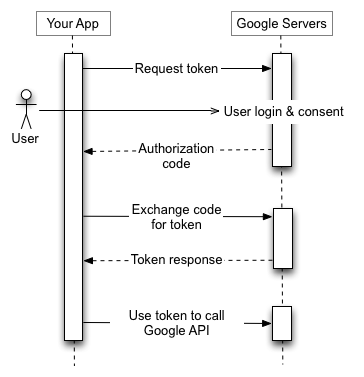
\includegraphics[width = 0.5\textwidth]{Imagenes/Bitmap/webflow.png}%
	\caption{OAuth 2.0 for Web Server Applications and Installed Applications.}%
	Image extracted from \cite{oauth}
	\label{fig:oauth}
\end{figure}

After constructing an \textit{InstalledAppFlow} by calling \textit{from\_client\_secrets\_file} as we have explained, we can invoke the class method \textit{run\_local\_server} which instructs the user to open the authorization URL in the browser and will try to automatically open it. This function will start a local web server to listen for the authorization response. Once there is a reply, the authorization server will redirect the user's browser to the local web server. As we can see in \ref{fig:oauth}, the web server will get the authorization code from the response and shutdown, that code is then exchanged for a token.

Then, we will be in possession of the OAuth 2.0 credentials for the user \citep{oauth2.credentials} which we are going to use for accessing the user's Gmail account. In summary, it is possible to obtain the necessary permissions from the user and to follow the OAuth 2.0 protocol, by executing these instructions (written in Python):

\begin{python}
from google_auth_oauthlib.flow import InstalledAppFlow

# Create a flow instance
flow = InstalledAppFlow.from_client_secrets_file('credentials.json', 
	['https://mail.google.com/'])
# Obtain OAuth 2.0 credentials for the user
creds = flow.run_local_server(port = 0)
\end{python}

Now, we are able to call Gmail API by using the token (which is stored in the variable \textit{creds}). However, before starting working on the email data, we should save the OAuth 2.0 credentials since otherwise the user would need to go through the consent screen every time the application is opened. To prevent the latter from happening, to differentiate access from mail management and consequently to reuse as much code as possible; we have implemented the following class \textit{auth}, in \textit{auth.py}, with a main method \textit{get\_credentials}:

\begin{pythonnum}
import pickle
import os.path
from google_auth_oauthlib.flow import InstalledAppFlow
from google.auth.transport.requests import Request
	
class auth:
	def __init__(self, SCOPES, CLIENT_SECRET_FILE):
		self.SCOPES = SCOPES
		self.CLIENT_SECRET_FILE = CLIENT_SECRET_FILE
	
	def get_credentials(self):
		"""
		Obtains valid credentials for accessing Gmail API
		"""
		creds = None
		# The file token.pickle stores the user's access and refresh tokens
		if os.path.exists('token.pickle'):
			with open('token.pickle', 'rb') as token:
				creds = pickle.load(token)
		# If there are no (valid) credentials available, let the user log in
		if not creds or not creds.valid:
			if creds and creds.expired and creds.refresh_token:
				creds.refresh(Request())
			else:
				flow = InstalledAppFlow.from_client_secrets_file(
					self.CLIENT_SECRET_FILE, self.SCOPES)
				creds = flow.run_local_server(port=0)
			# Create token.pickle and save the credentials for the next run
			with open('token.pickle', 'wb') as token:
				pickle.dump(creds, token)
		return creds

\end{pythonnum}

As we can observe in line 17 within \textit{get\_credentials} method, at first we check if the file called \textit{token.pickle} exists, and in that case, it is opened and its information is stored in the variable \textit{creds}. Thus, we avoid to force the user to open the authorization screen. By contrast, as we have seen before, if it does not exists, we obtain the credentials by calling the class methods \textit{from\_client\_secrets\_file} and \textit{run\_local\_server} (it is written between lines 25 and 30).

There is another case that is also reflected in the code above (in lines 23 and 24): the credentials are expired (it is possible to check it by executing \textit{creds.expired}) and they can be refreshed (the OAuth 2.0 refresh token is \textit{creds.refresh\_token}) \citep{oauth2.credentials}. In this situation, we will refresh the access token by invoking the method known as \textit{refresh} and by giving it a \textit{Request} object \citep{request-lib} from \textit{google.auth.transport.requests} as the function parameter which used to make HTTP requests.

\subsection{Building a Gmail Resource}
At this point, with the OAuth 2.0 credentials, we are able to call the Gmail API. For this purpose, it is necessary to construct a resource \citep[/v1/reference]{gmailAPI} for interacting with the API. The \textit{build} method, from \textit{googleapiclient.discovery} library \citep{build-module}, create that object. As we will see later, this resource will lead us to manage emails, drafts, threads and everything we will like to do with the user's Gmail data. This is why, using the \textit{auth.py} file explained in section \ref{ssect:oauth}, we are going to start every user session with the instructions below (or their equivalents in the language we are using):

\begin{python}
from googleapiclient.discovery import build
import auth

SCOPES = ['https://mail.google.com/']
CLIENT_SECRET_FILE = 'credentials.json'

# Creation of an auth instance
authInst = auth.auth(SCOPES, CLIENT_SECRET_FILE)
# Constructing the resource API object
service = build('gmail', 'v1', credentials = authInst.get_credentials())
\end{python}

Henceforth, we will use the \textit{service} variable to relate it with the resource object created by the \textit{build} method.

\subsection{Users resource}\label{ssect:userres}
The \textit{build} method could be called for obtaining any resource of any Google API (by giving it the suitable parameters). Our specific \textit{service} created\footnote{\url{http://googleapis.github.io/google-api-python-client/docs/dyn/gmail\_v1.html}} has an important instance method that we are going to invoke for every execution: \textit{users()} method. It returns what is known as users resource \citep[/v1/reference/users]{gmailAPI}.

The users resource has also instance methods, which return other Gmail API resources that we are going to need, such as \textit{drafts()}, \textit{labels()}, \textit{messages()} and \textit{threads()} which return drafts, labels, messages and threads resources respectively. Moreover, it possesses the three methods that we explain hereunder (we must remember that for being able to execute any method that we are going to explain in this and next sections, it is necessary to have the appropriate authorization with at least one of the required scopes that we can look up in its documentation):

\begin{itemize}
	\item\textit{getProfile(userId)}: it returns an object with a dictionary structure as it follows:
	\begin{python}
	{
	'threadsTotal' : integer, # Total number of threads in the mailbox
	'emailAddress' : string, # User's email address
	'historyId' : string, # ID of the mailbox's current history record
	'messagesTotal' : integer # Total number of messages in the mailbox
	}
	\end{python}
	The parameter is a string with the user's email address. If we remember the authentication process, at no time we ask the user about the email address because we decided to let the Google API functions to handle all that procedure. Therefore we have no way to know this information. Nevertheless, the special string value \textit{'me'} can be used to indicate the authenticated user. For knowing the required scopes for invoking this function look up in \cite[/v1/reference/users/getProfile]{gmailAPI}.
	\item\textit{stop(userId)}: stop receiving push notifications for the given user mailbox. As it happens with \textit{getProfile}, the parameter is a string with the user's email address, but it is possible to use the especial string value \textit{'me'}.
	\item\textit{whatch(userId, body)}: set up or update a push notification watch on the given user mailbox.
\end{itemize}

As we are going to call only the \textit{getProfile} method, we have described on details this first function and we have just given an idea about what the rest of them do. Now, in next sections, we are going to explain all the resources we can create with the user resource.

\subsection{Labels resource}\label{ssect:labres}
As we have seen in the explanation of users resource (section \ref{ssect:userres}), we can obtain labels resource \citep[/v1/reference/users/labels]{gmailAPI} by invoking \textit{labels()} instance method of our users resource, that is to say, by using our \textit{service} variable, the instruction \textit{service.users().labels()} will return the label resource.

Thanks to labels we are able to categorize messages and threads within the user's mailbox. They have a dictionary structure and their representation is what we can observe hereunder:

\begin{python}
{
'id' : string, # The immutable identifier of the label
'name' : string, # The display name
# The visibility of messages in the Gmail web interface
'messageListVisibility' : string,
'labelListVisibility' : string, # The visibility of label
'type' : string, # The owner type of the label ('system' or 'user')
'messagesTotal' : integer, # Total number of messages with the label
'messagesUnread' : integer, # Number of unread messages with the label
'threadsTotal' : integer, # Total number of threads with the label
'threadsUnread' : integer, # Number of unread threads with the label
'color' : {
	'textColor' : string, # Text color of the label, represented as hex string
	'backgroundColor' : string # Background color represented as hex string #RRGGBB
	}
}
\end{python}

The important fields we are going to need are the \textit{name} and the \textit{type}. Labels with \textit{system} type, such as \textit{INBOX}, \textit{SENT}, \textit{DRAFTS} and \textit{UNREAD}, are internally created and cannot be added, modified or deleted.

In order to obtain a label object, we will use the methods of this resource: create, delete, get, list, patch and update. In this manner, for example, we can store a label object by calling the next instructions:

\begin{python}
labels = service.users().labels()
labelList = labels.list(userId = 'me').execute()
label = labels.get(id = labelList[0]['id'], userId = 'me')
\end{python}

It is necessary to use the \textit{get} method because, as we can look up in \cite[/v1/reference/users/labels/list]{gmailAPI}, the \textit{list} method only contains an \textit{id}, \textit{name}, \textit{messageListVisibility}, \textit{labelListVisibility} and \textit{type} of each label, whereas the \textit{get} method returns the label resource with all the information.

\subsection{Messages resource}
In most of the operations we are going to execute, it will be essential the correct management of messages. Therefore, knowing how the emails are represented in Gmail API and how to use them is imperative to understand how to work with this API. For this reason, in this section we are going to delve into the messages resource of the Gmail API, its structure and its methods. As we saw in section \ref{ssect:userres}, we can access to this resource by invoking the \textit{messages()} method when we have a users resource.

\subsubsection{Resource representation}

Regardless of which programming language is used, messages resource \citep[/v1/reference/users/messages]{gmailAPI} internally has a dictionary structure as we can see down below:

\begin{python}
{
'id' : string,
'threadId' : string,
'labelIds' : [ string ],
'snippet' : string,
'historyId' : unsigned long,
'internalDate' : long,
'payload' : {
	'partId' : string,
	'mimeType' : string,
	'filename' : string,
	'headers' : [
		{
		'name' : string,
		'value' : string
		}
	],
	'body' : users.messages.attachments resource,
	'parts' : [ (MessagePart) ]
	},
'sizeEstimate' : integer,
'raw' : bytes
}
\end{python}

The more important keys (for us) of this data structure are (at least the most useful keys for our purpose):
\begin{itemize}
	\item\textit{id}: an immutable string which identifies the message.
	\item\textit{threadId}: we will explain the thread resource in \ref{ssect:threads} and we will see that a thread is composed of different messages that share common characteristics. The value of this field is a string which represent the identifier of the thread the message belongs to.
	\item\textit{labelIds}: a list of the identifiers of labels (see section \ref{ssect:labres}) applied to the message.
	\item\textit{payload}: as we can see in the resource representation above, it has a dictionary data structure. The \textit{payload} field is the parsed email structure in the message parts. The more important keys of the \textit{payload} field are:
	\begin{itemize}
		\item\textit{headers}: a list of headers. It contains the standard RFC 2822 \citep{rfc2822} email headers such as \textit{To}, \textit{From}, \textit{Subject} and \textit{Date}. Each header has a \textit{name} field, which is the name of the header (for example \textit{From}), and a \textit{value} field, which is the value of the header (following the same example as with the \textit{name} field: \textit{example@gmail.com} could be the value).
		\item\textit{parts}: a list which contains the different child MIME message parts (we will delve into this field in section \ref{sssect:mime}).
	\end{itemize}
	\item\textit{raw}: the entire email message in an RFC 2822 \citep{rfc2822} formatted and base64url (see section \ref{sssect:base64}) encoded string.
\end{itemize}

\subsubsection{Methods}
As any other resource we have studied and we will study, messages resource has a lot of methods, many of whom we are going to call for our purposes. We will limit ourselves to describing the methods we are going to use:

\begin{itemize}
	\item\textit{attachments()}: returns the attachments resource (see section \ref{ssect:attres})
	\item\textit{get(userId, id, format = 'full', metadataHeaders = None)}: if successful, this method returns the requested messages resource. Its parameters are:
	\begin{itemize}
		\item\textit{id}: the identifier string of the message we are looking for.
		\item\textit{userId}: the user's email address. As it happens with the \textit{getProfile} method of the users resource (see section \ref{ssect:userres}), the special string value \textit{'me'} can be used to indicate the authenticated user.
		\item\textit{format} (optional parameter): the format in which we want the message returned. This field can take the following punctual values: \textit{'full'} (returns the entirely email data with body content parsed in the \textit{payload} messages resource field and the \textit{raw} field is empty), \textit{'metadata'} (returns only an email message with its identifier, email headers and labels), \textit{'minimal'} (returns only an email message with its identifier and labels) and \textit{'raw'} (returns the entirely email message data with the body content in the \textit{raw} messages resource field as a base64url (see section \ref{sssect:base64}) encoded string and the \textit{payload} field is empty).
		\item\textit{metadataHeaders} (optional parameter): it is only used when the format parameter takes the punctual value of \textit{'metadata'}. It is a string list where we have to insert the headers we want to be included.
	\end{itemize}
	For knowing the required scopes for invoking this function look up in \cite[/v1/reference/users/messages/get]{gmailAPI}
	\item\textit{list(userId, includeSpamTrash = false, labelIds = None, maxResults = None, pageToken = None, q = None)}: returns a resource with the following structure:
	\begin{python}
		{
		'messages' : [ users.messages resource ],
		'nextPageToken' : string,
		'resultSizeEstimate' : unsigned integer
		}
	\end{python}
	As it happens with the \textit{list} method of the labels resource (see section \ref{ssect:labres}), \textit{'messages'} list does not contain all of a message information (for obtaining the full email data we can use \textit{get} method). Each element of this list only contains the \textit{id} and \textit{threadId} field.
	
	The parameters of this method are:
	\begin{itemize}
		\item\textit{userId}: user's email address (we can use the special string value \textit{'me'}).
		\item\textit{includeSpamTrash} (optional parameter): boolean parameter which determines if it includes messages with the labels \textit{SPAM} and \textit{TRASH} in the result of the operation.
		\item\textit{labelIds} (optional parameter): it is a list which let us filter the messages by only returning emails with labels that match all of the identifiers that belong to this list.
		\item\textit{maxResults} (optional parameter): an integer which determines the maximum number of messages to return.
		\item\textit{pageToken} (optional parameter): string which specifies a page of results.
		\item\textit{q} (optional parameter): string which let us do an specific query (with the same query format as the Gmail search box) and filter the messages by only returning emails that match with it.
	\end{itemize}
	For knowing the required scopes for invoking this function look up in \cite[/v1/reference/users/messages/list]{gmailAPI}
	\item\textit{send(userId, body = None, media\_body = None, media\_mime\_type = None)}: it sends the given message to the email addresses specified in the \textit{To}, \textit{Cc} and \textit{Bcc} headers. The first two parameters are the only ones we will use. The first (\textit{userId}) is the user's email address (we can use the special string value \textit{'me'}) and the second is the message we want to send in an RFC 2822 \citep{rfc2822} formatted. For knowing the required scopes for invoking this function look up in \cite[/v1/reference/users/messages/send]{gmailAPI}
\end{itemize}

\subsubsection{MIME} \label{sssect:mime}
To be able to create messages and read the body of the emails, it is essential to understand what the MIME standard consist of. Hence, in this section, we are going to give a general idea about this for, then, being able to draw on it in our development step.

MIME, whose acronym stands for Multipurpose Internet Mail Extensions \citep{wikimime}, is an Internet standard for the exchange of several file types (text, audio, video, etc.) which provides support to text with characters other than ASCII, non-text attachments, body messages with numerous pars (known as multi-part messages) and headers information with characters other than ASCII. Each data type has a different name in MIME. This names follows the format: type/subtype (both type and subtype are strings), in such a way that the first denotes the general data category and the second the specific type of that information. The values that the type can take are:

\begin{itemize}
	\item\textit{text}: means that the content is simple text. Subtypes like \textit{html}, \textit{xml} and \textit{plain} can follow this type.
	\item\textit{multipart}: indicates that the message has numerous parts with independent data. Subtypes like \textit{form-data} and \textit{digest} can follow this type.
	\item\textit{message}: it is used to encapsulate an existing message, for example when we want to reply a email and add the previous message. Subtypes like \textit{partial} and \textit{rfc822} can follow this type.
	\item\textit{image}: means that the content is an image. Subtypes like \textit{png}, \textit{jpeg} and \textit{gif} can follow this type.
	\item\textit{audio}: indicates that the content is an audio. Subtypes like \textit{mp3} and \textit{32kadpcm} can follow this type.
	\item\textit{video}: denotes that the content is an video. Subtypes like \textit{mpeg} and \textit{avi} can follow this type.
	\item\textit{application}: it is used for application data that could be binary. Subtypes like \textit{json} and \textit{pdf} can follow this type.
	\item\textit{font}: means that the content is a file which defines a font format. Subtypes like \textit{woff} and \textit{ttf} can follow this type.
\end{itemize}

MIME has several headers which are in all emails sent with this standard. Most important of them are the following:

\begin{itemize}
	\item\textit{Content-type}: the value of this header is the type and subtype of the message with the same structure that we have explained before. For example \textit{Content-Type: text/plain} means that the message is a plain text. By using the type \textit{multipart} make the creation of messages with parts and subparts organized in a tree structure (in which leaf nodes can belong to any type and the rest of them can belong to any multipart subtype variety) possible \citep{rfcmimemult}. A feasible composition of a message with a part with plain text and other non-text parts could be constructed by using \textit{multipart/mixed} as the root node like in figure \ref{fig:content-type}. Indeed, in the example of the figure \ref{fig:content-type}, we can observe the use of \textit{multipart/alternative} for a message which contains the body both in plain text and in html text. Other different emails constructions are possible (like forwarding with the original message attached by using \textit{multipart/mixed} with a \textit{text/plain} part and a \textit{message/rfc822} part) thanks to the tree structure of the \textit{Content-type} header.
	
	Another important detail, that we can repair by observing the message example in figure \ref{fig:content-type}, is the fact that each node of the tree structure of the emails is visited and showed following the pre-order traversal.
	
	\begin{figure}[t]
		\centering%
		\includegraphics[width = 1.2\textwidth]{Imagenes/Bitmap/tree-content-type.png}%
		\caption{MIME types tree structure of an email example}%
		\label{fig:content-type}
	\end{figure}
	\item\textit{Content-Disposition}: this header is used to indicate the presentation style of the part of the message. There are two ways to show the part: \textit{inline} content-disposition (which means that the content must be displayed at the same time as the message) and \textit{attachment} content-disposition (the part is not displayed at the same time as the message and it requires some form or action from the user to see it). Furthermore, this header also provides several fields for specifying other type of information about the content, such as the name of the file and the creation or modification date. The following example is taken from \cite{rfc2183} (and, as we will explain after the example, it does not match with the syntax of this same header in the example that we can see in the last part of the example message of figure \ref{fig:content-type}):
	\begin{lstlisting}
		Content-Disposition: attachment; filename=genome.jpeg;
			modification-date="Wed, 12 Feb 1997 16:29:51 -0500";
	\end{lstlisting}
	As we have said, this syntax is different from the used in the email example of the figure \ref{fig:content-type}. This results from the fact that, in HTTP, the header we find in that figure (\textit{Content-Disposition: attachment}) is usually used for instructing the client to show the response body as a downloadable file. As we can observe, it has a \textit{filename} field which is used for establishing the default file name when the user is going to download it.
	
	\item\textit{Content-Transfer-Encoding}: when we want to send some files in a message, sometimes they are represented as 8-bit character or binary data, which are not allowed in some protocols. On this account, it is necessary to have a standard that indicates how we should re-encoding such data into a 7-bit short-line format. The Content-Transfer-Encoding header \citep{w3cte} will tell the client which transformation has been used for being able to transport that data. Therefore and for lack of a previous standard which states a single Content-Transfer-Encoding mechanism, the possible values, which specify the type of encoding, this header can take are: \textit{'base64'} (see section \ref{sssect:base64}), \textit{'quoted-printable'} (see section \ref{sssect:quot-p}), \textit{'8bit'}, \textit{'7bit'}, \textit{'binary'} and \textit{'x-token'}. All these values are not case sensitive. If this header does not exist, we can assume that the value of this header is \textit{'7bit'}, which means that the body of the message is already in a seven-bit mail-ready representation, in other words, all the body of the message is represented as short lines of US-ASCII data. Despite the \textit{'8bit'}, \textit{'7bit'} and \textit{'binary'} indicate that the content has not been transformed, they are useful for knowing the kind of encoding that the data has. This header will generally be omitted when the Content-Type has the \textit{multipart} or \textit{'message'} type (as it happens in the message example of the figure \ref{fig:content-type}), because it also admits the last three types we have mentioned.
	
	It is common to add another header (as we can see in figure \ref{fig:content-type}) called \textit{charset}, which value instructs the client the original encoding of data for, then, being able to decode it.
\end{itemize}

\subsubsection{Base64} \label{sssect:base64}

\subsubsection{Quoted-printable} \label{sssect:quot-p}

\subsection{Attachments resource} \label{ssect:attres}

\subsection{Threads resource}\label{ssect:threads}

%Drafts resource
%Limitaciones de la API
\chapter{Style Analyser}
\label{cap:analyser}

In order to generate messages with the user's writing style, it is necessary to define parameters which will determine and describe it. For this purpose, we have developed a style analyser that extracts the messages written by the user and obtains the value of various metrics from them. Then it will be useful for analysing different user's emails and drawing conclusions about what parameters describe the writing style of each person more accurately.

In this section we are going to explain the architecture of this analyser (see Section \ref{section:stylearch}) and each of the modules that compose it (they are explained in Sections \ref{section:extmod}, \ref{section:prepmod}, \ref{section:typomod} and \ref{section:measmod}). Finally, we are going to discuss the obtained results and analyse them for drawing a conclusion (this discussion can be looked up in \ref{section:resconc}).

\section{Architecture} \label{section:stylearch}
The first step when we are designing a system's architecture is to know its input and output. In this case, we want to implement a natural language processing system that analyses the writing style of e-mails. As we have previously mentioned, the stylometric analysis will be represented through chosen style markers. Therefore, our system's output is going to be that chosen metrics (they are explained in section \ref{section:measmod}) of each message.

In respect of the system's input, because of the nature of the problem we face, it is reasonable to think that it must be an e-mail. However, we do not have the corpus of e-mails to analyse. For this reason, our first step will be to extract the e-mails that will be analysed. Hence, our system's input is going to be the information of the Gmail user for accessing to the data that we are interested in. Therefore, we are going to develop a system which receives some information of a Gmail user as input and obtains different metrics for each message sent by the given user as output.

Once we clearly know the input and output of our system, we need to define the different steps that a message have to take for being analysed. In this manner, we are going to design a pipeline architecture with four different phases (extraction, preprocessing, typographic correction and measuring) as Figure \ref{fig:arch} shows. Thus, we divide the original job in four different and more simple tasks with distinct inputs and outputs required. This division into phases addresses both the need to atomise each of the steps to obtain the desired output, and to take advantage of benefits that a single indivisible system does not provide. One of these advantages is the possibility of working in parallel with each of the different phases. Another advantage, without a doubt, is the greater facility for the correction of errors in the pipeline. Thus, if an error of any kind is found in any phase, this will not affect the implementation of subsequent phases and it will not be necessary to modify the entire system. This, together with the fact that each phase stores its corresponding output using different Mongo DB documents (see Section \ref{sect:mongo}), allows us to change the behaviour of a phase (either in case of improvement or error correction of the implementation) avoiding to execute again the previous phases to the modified one, it would only be necessary to execute the changed phase and the ones that follow. Finally, it is also important to note the advantage of reusing each of the phases separately without having to rely on the others.

\begin{figure}[h]
	\centering%
	\centerline{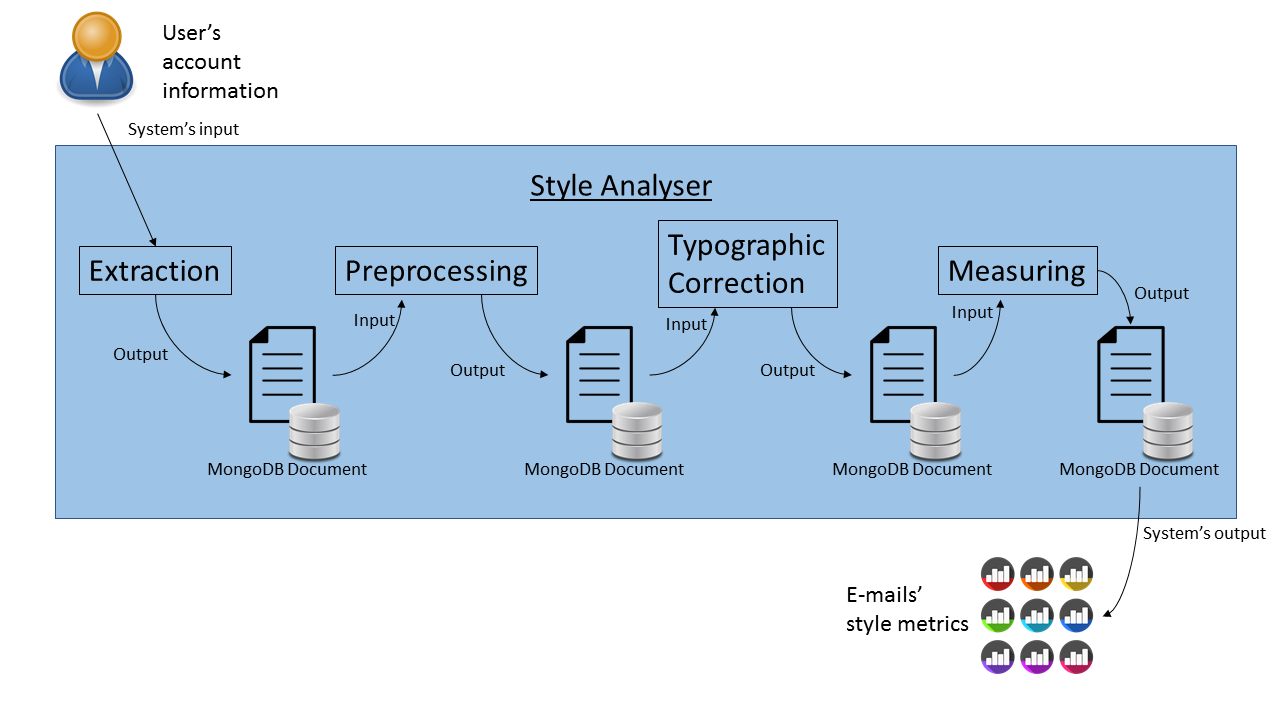
\includegraphics[width = 1.2\textwidth]{Imagenes/Bitmap/Analyser/architecture.png}}%
	\caption{Pipeline architecture of the style analyser}%
	\label{fig:arch}
\end{figure}

As it is easy to deduce, each of these phases is going to be developed as a different module. This implementation will have the advantage that each module is going to be able to work independently from the other modules, which will allow them to work in parallel. That is to say, while a message is being extracted, other e-mails could be being preprocessed, corrected or measured if they have gone through the previous phases. This optimizes the time it takes for a message to be extracted until the respective metrics are calculated (it does not have to wait for the others to move to the next phase of the pipeline). In addition, the last three (preprocessing, typographic correction and measuring) have been implemented as web services using Flask (see Section \ref{sect:flask}), which facilitates their reuse even separately in other works and projects. Let us now briefly explain what each of the defined phases consists of.

The first step, extraction phase, consists of the extraction of each one of the sent messages of the given user. In this task, we are going to take advantage of all the studied concepts about the Gmail API (see Section \ref{ssect:gmailapi}) and make use of every resource it provides us. Besides, we will try to minimize the consumed quota units in each extraction, which means we will only make the requests to the Google Servers that are strictly necessary. This first step is not just the task of extracting the resource that represents each sent message from the user's account, but also the job of transforming it to the format that the preprocessing module needs. Hence, the input of this module will be the same input as that of the complete system (information about Gmail user) and its output will be an extracted message ready for being preprocessed.

As for the second step, the preprocessing phase, consists of modifying the extracted message so that it can be interpreted by the spaCy's natural language processing model to be used. Some of the changes that a message could suffer in this phase are: the removal of the signature, the disposal of the replied messages which appears under the text, the elimination of soft break lines that quoted-printable codification (see Section \ref{sssect:quot-p}) introduce in some messages, etc. This module also addresses the need to remove characters and structures that do not correspond to those used in a plain text such as bold or italic type styles, font sizes and fonts, enumerations or bulleted lists, etc. Likewise, its output is a message with its body as a plain text.

In the implemented metrics (as we will see in section \ref{section:measmod}) we will not take into account typographical errors (such as a spelling mistake). So we will need to fix them as much as possible, and this is the typographic correction module's task. In the same way, it is possible that some tokens do not belong to our spaCy model's vocabulary. Therefore, it will be necessary to know lexical-syntactic information about the token, such as its part of speech and its lemma. These are the task of the typographic correction module.

Finally, the measuring module is in charge of calculating all the style features chosen for this work. For that purpose, it receives a message (extracted by the extracting module) with a plain text format (thanks to the preprocessing module) free from typographic error (thanks to the typographic correction module) and obtains the result of measuring all the style markers selected in the given message.

As we have explained, the input of the extracting module is information about a Gmail user and the input of the rest of the modules is a single message. However, each module is independent from each other, which means that it is necessary to have a way of assembling all this modules. For this purpose, the \textit{Analyser} class is developed (see Section \ref{sect:analyserclass}). This entity is in charge of sending to each module the required input in order to obtain its output. Moreover, it presents the system to the user, communicates the information and captures the user's information (it performs a previous filtering to check that there are no formatting errors), such as the typographic correction of the errors found. In this manner, the architecture of our style analyser system is as shown in Figure \ref{fig:umlarch} (in the following sections we will delve into each module of this system), which represents the UML (Unified Modelling Language) class diagram of it. In this figure we have avoided including both attributes and methods of each class, since with it we want to show the general structure of the system. In the sections corresponding to each of the packages and the \textit{Analyser} class, their attributes and methods will be specified and explained.

\begin{figure}[p]
	\centering%
	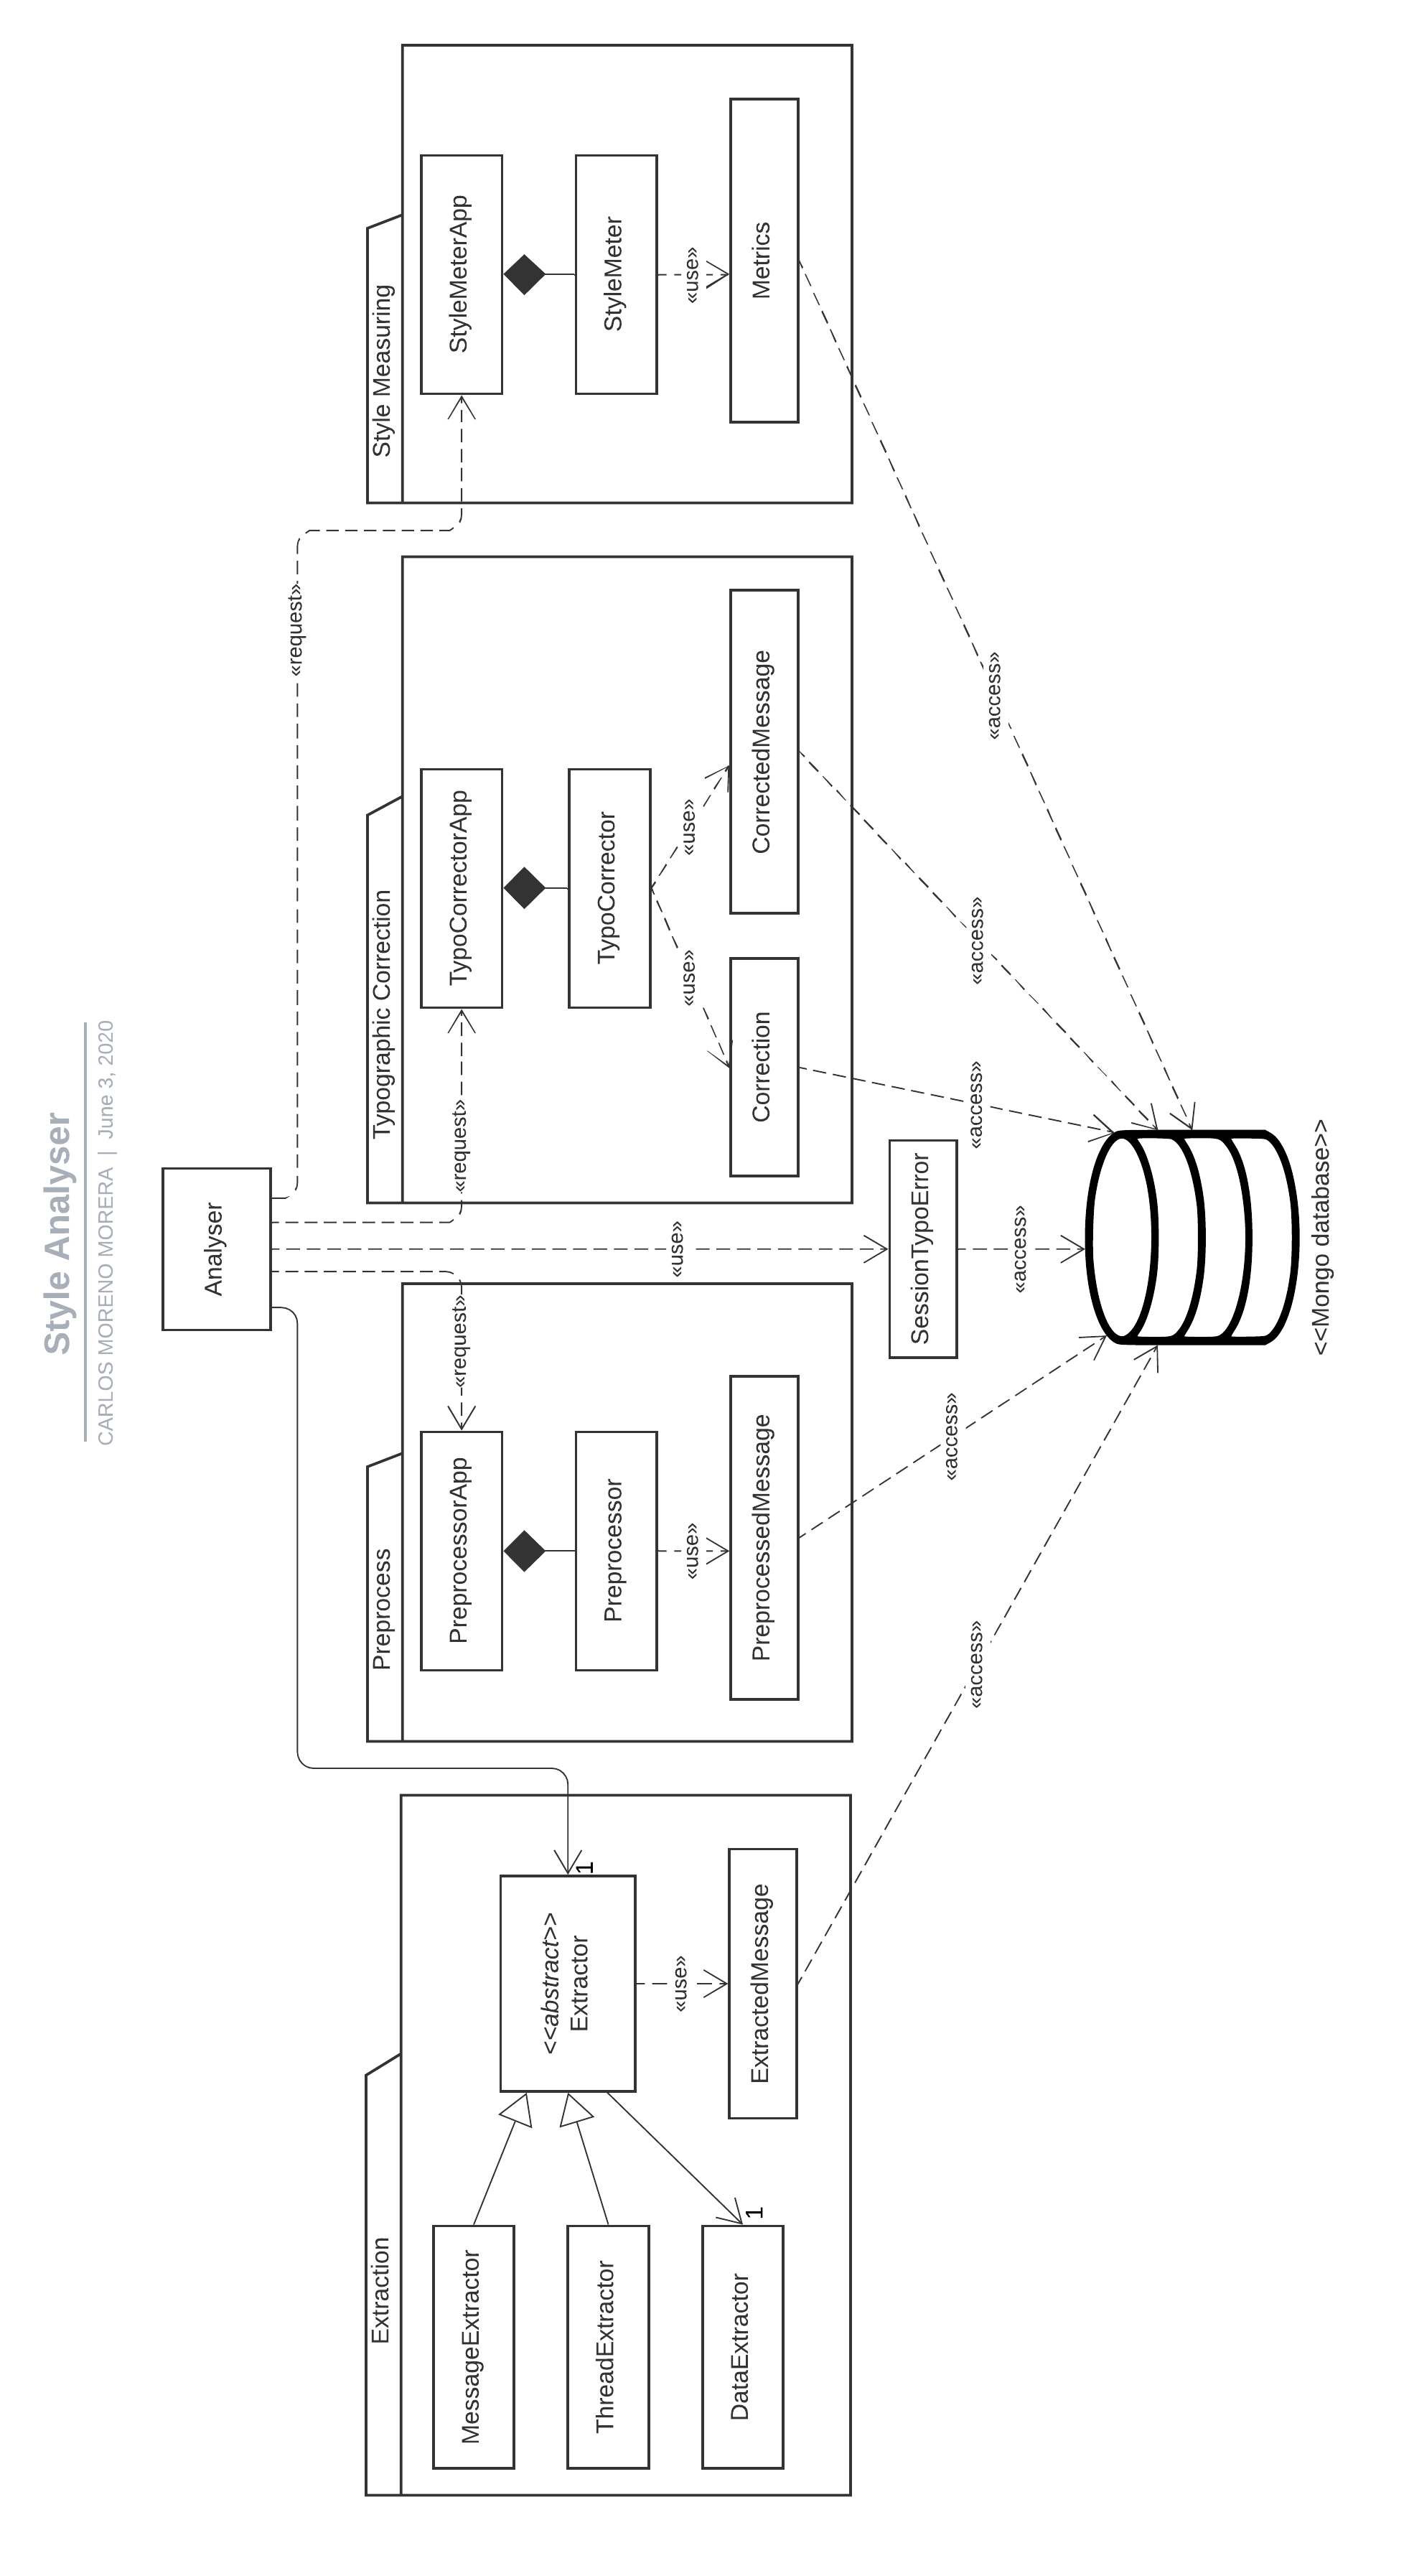
\includegraphics[height=0.85\paperheight]{Imagenes/Bitmap/Analyser/StyleAnalyserUML.png}%
	\caption{UML class diagram of the style analyser}%
	\label{fig:umlarch}
\end{figure}

As we wanted, the \textit{Analyser} manages the communication between each UML package (which represent each of the mentioned modules). Thus, this UML class will transport the output of each module to the input of the subsequent phase so as to fulfil the pipeline established in Figure \ref{fig:arch}.

If we look at the relationship shared by the \textit{Analyser} class and the \textit{Extraction} package (specifically with the \textit{Extractor} class of this module), we will notice that it is an uni-directional binary association, what it means that the objects of the second are connected with the objects of the first. Furthermore, we can observe a multiplicity index in the arrowhead (the \textit{Extraction}'s end), which means that the \textit{Analyser} will be related with an only \textit{Extractor} object (it will not be necessary to have more than one \textit{Extraction} package in order to obtain all user's sent messages).

The rest of packages are ``used'' by the \textit{Analyser}, through a POST HTTP request, because all of them are implemented as web services. It contacts with the module's app which is related with the module's main class (which is in charge of carrying out its corresponding task).

An important observation to mention is the fact that all packages interact with their corresponding classes, which act as DAO (Data Access Object), with the database used (with Mongo DB technology as it is explained in Section \ref{sect:mongo}). Their interaction is based on storing their results in it. The main advantage of this implementation is that it is not required to have enough dynamic memory in order to process every message at the same time. In addition to it, as we have explained, if an error is detected in an specific phase, it is not necessary to execute the previous modules again. With this in mind, it is reasonable to think that each module's main class, of the last three phases, will make use of the corresponding class with the purpose of saving its result, obviously after finishing its execution with the given message.

Below we only have to enter in detail of each of the packages and of the \textit{Analyser}, in order to completely understand the style analyser.

\section{Extracting Module} \label{section:extmod}

\section{Preprocessing Module} \label{section:prepmod}

\section{Typographic Correction Module} \label{section:typomod}

\section{Measuring module} \label{section:measmod}

As in our case we have used 31 lexical-syntactic features (due to previous studies, such as \cite{homem2011authorship}, yield encouraging results with lexical-syntactic features), following the classification of \cite{abbasi2008writeprints} (which categorised stylistic features as lexical, syntactic, structural, content-specific and idiosyncratic style markers), we will now divide them into 4 categories in which we have grouped them according to their usefulness in terms of what type of conclusions we can infer from each of them. These categories are: part of speech features (see Section \ref{ssect:posf}), punctuation features (see Section \ref{ssect:punctf}), vocabulary features (see Section \ref{ssect:vocabf}) and structural features (see Section \ref{ssect:strucf}). We must not confuse this latter category (which it belongs to the lexical features of the classification given in \cite{abbasi2008writeprints}) with the structural metrics explained in \cite{abbasi2008writeprints}.

Some of the popular metrics which are not used in this work, belong to the structural, content-specific and idiosyncratic style markers of \cite{abbasi2008writeprints}, but there are others which belong to the same categories as the explained metrics (lexical and syntactic).

The choice of the metrics presented below, some essentially simple, has been directed by the objective of finding easily explainable characteristics that set the parameters of the style of writing according to the recipient of the email, and then be able to use this study to develop, in future projects, systems of natural language generation of emails that take into account this factor. For this reason, some excessively complex metrics, although popular in stylometry, have been avoided and an attempt has been made to prioritize the explainability of the chosen features.

\subsection{Part of Speech features}\label{ssect:posf}

We will call our part of speech metrics as the syntactic features which have to do with the part of speech of each word of the e-mails. Following the suggestion of \cite{holmes1985analysis}, we count the number of nouns, verbs, adjectives, adverbs, pronouns, determinants, conjunctions and prepositions of each text. By calculating this, significant stylistic traits may be found, because as \cite{somers1966statistical} claims: ``A more cultivated intellectual habit of thinking can increase the number of substantives used, while a more dynamic empathy and attitude can be habitually expressed by means of an increased number of verbs. It is also possible to detect a number of idiosyncrasies in the use of prepositions, subordinations, conjunctions and articles''.

In adding to this metrics, we calculate the verb-adjective ratio and the determinant-pronouns ratio, extracted from \cite{antosch1969diagnosis} and \cite{brainerd1974weighting}, respectively.

\subsection{Punctuation features}\label{ssect:punctf}

In order to extract conclusions from this syntactic features, and following the example of \cite{calix2008stylometry}, we calculate the amount of commas, periods, semi-colons, ellipsis and pair of brackets. With these metrics we can reach conclusions such as the structural complexity of a message (since, for example, juxtaposition structures appear in the presence of some of these scores), the division into sentences of the message or the need for clarification of the text transmitted (for example, by analysing the amount of brackets).

\subsection{Vocabulary features}\label{ssect:vocabf}

In terms of the vocabulary used, we work with the ``bag of words'' metrics, in other words, we note how many times each different word is used in a message. Of course this is not the only metric that we can categorise as a vocabulary feature and from which we can extract conclusions about the vocabulary used. There are many other which tries to set the parameters of, for instance, the difficult of the vocabulary or its richness. Besides, from the computing of the bag of words, we are able to easily obtain other style marker chosen which also belongs to this category of vocabulary features: the amount of different words in each text, proposed in \cite{ril2014determination} and in \cite{corney2001identifying}.

As for the difficulty level, it determines the level of education that someone needs to have if they are to understand the text. There are several indices available to calculate this level, such as the proposed in \cite{dale1948formula}, the Gunning Fog Index \citep{wiki:gunning} or the Flesch-Kincaid index \citep{dubay2004principles}, although the latter is the most commonly documented and cited. The expression which determines the Flesch-Kincaid index is the following:

$$
I_{FK} = 1.599\lambda-1.015\beta-31.517
$$

Where $\lambda$ is the mean of one-syllable words per 100 words, and $\beta$ is the mean sentence length measured by the number of words. However, as our spaCy's pretrained Spanish model (see Section \ref{sect:spacy}) is not able to divide words by syllables, we determine $\lambda$ as the mean of words with two or less characters per 100 words.

In respect of the richness of the vocabulary, we have chosen two different metrics. The first that we are going to explain is the one proposed by \cite{honore1979some}, which determines the richness of te vocabulary based on the total unrepeated words used in the text. The following formula defines it:

$$
R_H = \frac{100\log(M)}{M^2}
$$

Where $M$ is the number of different words in the text. However, as \cite{ril2014determination} claims, depending on the type of document being analysed, the calculation of $R_H$ has more or less validity (for instance, certain specialist articles, as their nature, requires constant repetition of words). As a consequence of this, another definition of richness of vocabulary is proposed by \cite{yule2014statistical}. This richness marker, that we are going to use as our second richness of vocabulary style marker, is called Yule's characteristic and defined with the following expression:

$$
K = \frac{10^4\left(\sum_{i = 1}^\infty i^2V_i-M\right)}{M^2}
$$

Where $M$ is the number of different words in the text and $V_i$ is the number of words that appear i times in the document.

From Yule's Characteristic we are able to calculate the Simpson's Index (denoted as $D$), defined in \cite{simpson1949measurement}. This famous metric is understood as the measurement of diversity based on the change that the two members of an arbitrary chosen pair of word tokens will belong to the same type. To calculate $D$ it is necessary to divide the total number of identical pairs in the sample by the number of all possible pairs, that is to say, what the following expression defines:

$$
D = \frac{\sum_{i = 1}^\infty i(i-1)V_i}{M(M-1)}
$$

Where we are maintaining the Yule's Characteristic notation. However, as we have transmitted in advance, it is possible to calculate the Simpson's Index if we know the value of Yule's Characteristic. This relationship is defined by the following expression (and we are going to use it in the implementation in order to speed the computing):

$$
10^{-4}K=D\left(1-\frac{1}{M}\right)
$$

Vocabulary distribution can also be measured by using a concept linguists have borrowed from thermodynamics and applied to communication theory: entropy (used in \cite{holmes1985analysis}). In literary text it is true that with an increase in internal structure, entropy decreases, and with an increase in disorder or randomness, the measure of entropy increases. The expression for the entropy of a system (vocabulary in this case) is:

$$
H = -\sum_{i=1}^{\infty} p_i\log(p_i)
$$

Where $p_i$ is the probability of appearance of the ith lemma (found by dividing the number of occurrences of that lemma by the total number of words in the text). Due to the value will change according to how much text is analysed, the formula may be refined in order that works of different length may be compared. In this way, as it is proposed in \cite{holmes1985analysis}, the following expression determines absolute diversity for any length text as 100, while absolute uniformity remains zero:

$$
H=-100\sum_{i = 1}^{\infty}p_i\frac{\log(p_i)}{\log(M)}
$$

In addition to the words distribution features (which are the bag of words and the amount of different words), the level of difficulty, the richness of vocabulary (which is measured by the formula proposed in \cite{honore1979some} and the Yule's Characteristic), the diversity (represented by the Simpson's Index) and the internal structure of the vocabulary (which is measured by the entropy), we have defined other four style markers which also allow us to extract conclusions about some feature of the vocabulary of the message. First of these is the most popular and old style marker: the mean word length. Researches as \cite{ril2014determination} claim that it is ``directly connected with the richness of the author's vocabulary and measures his or her ability to use complex words'', due to it is considered that complex words are formed by three or more syllables that do not represent proper nouns, prefixes, suffixes or compound words. Thus, \cite{ril2014determination} propose an expression similar to the following one in order to calculate it:

$$
L_W = \frac{\sum_{i=1}^{\infty}i*C_i}{N}\cdot 100
$$

Where $C_i$ is the number of words with $i$ characters and $N$ is the number of words used. This formula is analogous to the expression proposed by \cite{ril2014determination}, except that with the one that we have presented the punctuation marks are removed from the numerator.

The second of these writing style metrics is the measurement of words length frequency distribution, that is to say, how many words with one character appears in the document, with two characters and so on up to the length of the longest word. Despite of being strongly influenced by the language, it is used in researches as \cite{corney2001identifying} and \cite{kemp1976personal}, as it is claimed in\cite{allen1974methods}, ``Each writer, however, will have his own curve, so that although English (and German) texts in general peak at three letters, the writings of John Stuart Mill peak at two and those of Shakespeare peak at four''. Our interest will then focus on checking whether, in addition to depending on the author, this metric varies according to the recipient of the email.

The rest of vocabulary features are related to the stop words present in the text. The simplest of those metrics is the style marker which consists of calculating the total number of stop words (denoted as $T_S$). On the other hand, as it is proposed in \cite{ril2014determination},  we will calculate the stop words ratio, which is defined with the following expression:

$$
S_W = \frac{T_S}{N}\cdot 100
$$

\subsection{Structural features}\label{ssect:strucf}

We will denote by structural features those characteristics that we obtain directly from the construction of the analysed text. Some of these metrics are as simple as the total number of characters in the body of the email or the absolute number of words in the email, both used in researches such as in \cite{corney2001identifying} and \cite{ril2014determination}.

Most of these features are sentence length dependent. Both \cite{tallentire1972appraisal} and \cite{kjetsaa1979and} agree that summary measures such as average sentence-lengths are of little use in stylometry studies but distributions of sentence-lengths can be useful, even on their own. Taking into account the above, we will find both the distribution of the length of the sentences (calculated in number of characters and number of words) and the average length of the sentences in a message found by the number of words, as it is proposed in \cite{corney2001identifying}. For the first one, we are going to store the number of sentence with length one, two, three and so on up to the length of the longest one, by measuring it  using both the number of characters and the number of words.

\section{Results and conclusions} \label{section:resconc}

%\include{Capitulos/Capitulo4}
%\include{Capitulos/Capitulo5}
\chapter{Conclusiones y Trabajo Futuro}
\label{cap:conclusiones}

\chapterquote{Difficult to see. Always in motion is the future.}{Yoda - Star Wars: Episode III – Revenge of the Sith (2005)}

Conclusiones del trabajo y líneas de trabajo futuro.

Antes de la entrega de actas de cada convocatoria, en el plazo que se indica en el calendario de los trabajos de fin de máster, el estudiante entregará en el Campus Virtual la versión final de la memoria en PDF. En la portada de la misma deberán figurar, como se ha señalado anteriormente, la convocatoria y la calificación obtenida. Asimismo, el estudiante también entregará todo el material que tenga concedido en préstamo a lo largo del curso.




%%%%%%%%%%%%%%%%%%%%%%%%%%%%%%%%%%%%%%%%%%%%%%%%%%%%%%%%%%%%%%%%%%%%%%%%%%%
% Si el TFM se escribe en inglés, comentar las siguientes líneas 
% porque no es necesario incluir nuevamente las Conclusiones en inglés
\begin{otherlanguage}{english}
\chapter{Introduction}
\label{cap:introduction}

Introduction to the subject area. This chapter contains the translation of Chapter \ref{cap:introduccion}.










\chapter{Conclusions and Future Work}
\label{cap:conclusions}

Conclusions and future lines of work. This chapter contains the translation of Chapter \ref{cap:conclusiones}.



\end{otherlanguage}
%%%%%%%%%%%%%%%%%%%%%%%%%%%%%%%%%%%%%%%%%%%%%%%%%%%%%%%%%%%%%%%%%%%%%%%%%%%

%
% Bibliografía
%
% Si el TFM se escribe en inglés, editar TeXiS/TeXiS_bib para cambiar el
% estilo de las referencias
%---------------------------------------------------------------------
%
%                      configBibliografia.tex
%
%---------------------------------------------------------------------
%
% bibliografia.tex
% Copyright 2009 Marco Antonio Gomez-Martin, Pedro Pablo Gomez-Martin
%
% This file belongs to the TeXiS manual, a LaTeX template for writting
% Thesis and other documents. The complete last TeXiS package can
% be obtained from http://gaia.fdi.ucm.es/projects/texis/
%
% Although the TeXiS template itself is distributed under the 
% conditions of the LaTeX Project Public License
% (http://www.latex-project.org/lppl.txt), the manual content
% uses the CC-BY-SA license that stays that you are free:
%
%    - to share & to copy, distribute and transmit the work
%    - to remix and to adapt the work
%
% under the following conditions:
%
%    - Attribution: you must attribute the work in the manner
%      specified by the author or licensor (but not in any way that
%      suggests that they endorse you or your use of the work).
%    - Share Alike: if you alter, transform, or build upon this
%      work, you may distribute the resulting work only under the
%      same, similar or a compatible license.
%
% The complete license is available in
% http://creativecommons.org/licenses/by-sa/3.0/legalcode
%
%---------------------------------------------------------------------
%
% Fichero  que  configura  los  parámetros  de  la  generación  de  la
% bibliografía.  Existen dos  parámetros configurables:  los ficheros
% .bib que se utilizan y la frase célebre que aparece justo antes de la
% primera referencia.
%
%---------------------------------------------------------------------


%%%%%%%%%%%%%%%%%%%%%%%%%%%%%%%%%%%%%%%%%%%%%%%%%%%%%%%%%%%%%%%%%%%%%%
% Definición de los ficheros .bib utilizados:
% \setBibFiles{<lista ficheros sin extension, separados por comas>}
% Nota:
% Es IMPORTANTE que los ficheros estén en la misma línea que
% el comando \setBibFiles. Si se desea utilizar varias líneas,
% terminarlas con una apertura de comentario.
%%%%%%%%%%%%%%%%%%%%%%%%%%%%%%%%%%%%%%%%%%%%%%%%%%%%%%%%%%%%%%%%%%%%%%
\setBibFiles{%
biblio%
}

%%%%%%%%%%%%%%%%%%%%%%%%%%%%%%%%%%%%%%%%%%%%%%%%%%%%%%%%%%%%%%%%%%%%%%
% Definición de la frase célebre para el capítulo de la
% bibliografía. Dentro normalmente se querrá hacer uso del entorno
% \begin{FraseCelebre}, que contendrá a su vez otros dos entornos,
% un \begin{Frase} y un \begin{Fuente}.
%
% Nota:
% Si no se quiere cita, se puede eliminar su definición (en la
% macro setCitaBibliografia{} ).
%%%%%%%%%%%%%%%%%%%%%%%%%%%%%%%%%%%%%%%%%%%%%%%%%%%%%%%%%%%%%%%%%%%%%%
\setCitaBibliografia{
\begin{FraseCelebre}
\begin{Frase}
  Y así, del mucho leer y del poco dormir, se le secó el celebro de
  manera que vino a perder el juicio.\\ 
  \textcolor{red}{(modificar en Cascaras$\backslash$bibliografia.tex)}
\end{Frase}
\begin{Fuente}
  Miguel de Cervantes Saavedra
\end{Fuente}
\end{FraseCelebre}
}

%%
%% Creamos la bibliografia
%%
\makeBib

% Variable local para emacs, para  que encuentre el fichero maestro de
% compilación y funcionen mejor algunas teclas rápidas de AucTeX

%%%
%%% Local Variables:
%%% mode: latex
%%% TeX-master: "../Tesis.tex"
%%% End:



% Apéndices
\appendix
\chapter{Título del Apéndice A}
\label{Appendix:Key1}

Contenido del apéndice
\chapter{Título del Apéndice B}
\label{Appendix:Key2}

%\include{Apendices/appendixC}
%\include{...}
%\include{...}
%\include{...}
\backmatter



%
% Índice de palabras
%

% Sólo  la   generamos  si  está   declarada  \generaindice.  Consulta
% TeXiS.sty para más información.

% En realidad, el soporte para la generación de índices de palabras
% en TeXiS no está documentada en el manual, porque no ha sido usada
% "en producción". Por tanto, el fichero que genera el índice
% *no* se incluye aquí (está comentado). Consulta la documentación
% en TeXiS_pream.tex para más información.
\ifx\generaindice\undefined
\else
%%---------------------------------------------------------------------
%
%                        TeXiS_indice.tex
%
%---------------------------------------------------------------------
%
% TeXiS_indice.tex
% Copyright 2009 Marco Antonio Gomez-Martin, Pedro Pablo Gomez-Martin
%
% This file belongs to TeXiS, a LaTeX template for writting
% Thesis and other documents. The complete last TeXiS package can
% be obtained from http://gaia.fdi.ucm.es/projects/texis/
%
% This work may be distributed and/or modified under the
% conditions of the LaTeX Project Public License, either version 1.3
% of this license or (at your option) any later version.
% The latest version of this license is in
%   http://www.latex-project.org/lppl.txt
% and version 1.3 or later is part of all distributions of LaTeX
% version 2005/12/01 or later.
%
% This work has the LPPL maintenance status `maintained'.
% 
% The Current Maintainers of this work are Marco Antonio Gomez-Martin
% and Pedro Pablo Gomez-Martin
%
%---------------------------------------------------------------------
%
% Contiene  los  comandos  para  generar  el índice  de  palabras  del
% documento.
%
%---------------------------------------------------------------------
%
% NOTA IMPORTANTE: el  soporte en TeXiS para el  índice de palabras es
% embrionario, y  de hecho  ni siquiera se  describe en el  manual. Se
% proporciona  una infraestructura  básica (sin  terminar)  para ello,
% pero  no ha  sido usada  "en producción".  De hecho,  a pesar  de la
% existencia de  este fichero, *no* se incluye  en Tesis.tex. Consulta
% la documentación en TeXiS_pream.tex para más información.
%
%---------------------------------------------------------------------


% Si se  va a generar  la tabla de  contenidos (el índice  habitual) y
% también vamos a  generar el índice de palabras  (ambas decisiones se
% toman en  función de  la definición  o no de  un par  de constantes,
% puedes consultar modo.tex para más información), entonces metemos en
% la tabla de contenidos una  entrada para marcar la página donde está
% el índice de palabras.

\ifx\generatoc\undefined
\else
   \addcontentsline{toc}{chapter}{\indexname}
\fi


% Generamos el índice
\printindex

% Variable local para emacs, para  que encuentre el fichero maestro de
% compilación y funcionen mejor algunas teclas rápidas de AucTeX

%%%
%%% Local Variables:
%%% mode: latex
%%% TeX-master: "./tesis.tex"
%%% End:

\fi

%
% Lista de acrónimos
%

% Sólo  lo  generamos  si  está declarada  \generaacronimos.  Consulta
% TeXiS.sty para más información.


\ifx\generaacronimos\undefined
\else
%---------------------------------------------------------------------
%
%                        TeXiS_acron.tex
%
%---------------------------------------------------------------------
%
% TeXiS_acron.tex
% Copyright 2009 Marco Antonio Gomez-Martin, Pedro Pablo Gomez-Martin
%
% This file belongs to TeXiS, a LaTeX template for writting
% Thesis and other documents. The complete last TeXiS package can
% be obtained from http://gaia.fdi.ucm.es/projects/texis/
%
% This work may be distributed and/or modified under the
% conditions of the LaTeX Project Public License, either version 1.3
% of this license or (at your option) any later version.
% The latest version of this license is in
%   http://www.latex-project.org/lppl.txt
% and version 1.3 or later is part of all distributions of LaTeX
% version 2005/12/01 or later.
%
% This work has the LPPL maintenance status `maintained'.
% 
% The Current Maintainers of this work are Marco Antonio Gomez-Martin
% and Pedro Pablo Gomez-Martin
%
%---------------------------------------------------------------------
%
% Contiene  los  comandos  para  generar  el listado de acrónimos
% documento.
%
%---------------------------------------------------------------------
%
% NOTA IMPORTANTE:  para que la  generación de acrónimos  funcione, al
% menos  debe  existir  un  acrónimo   en  el  documento.  Si  no,  la
% compilación  del   fichero  LaTeX  falla  con   un  error  "extraño"
% (indicando  que  quizá  falte  un \item).   Consulta  el  comentario
% referente al paquete glosstex en TeXiS_pream.tex.
%
%---------------------------------------------------------------------


% Redefinimos a español  el título de la lista  de acrónimos (Babel no
% lo hace por nosotros esta vez)

\def\listacronymname{Lista de acrónimos}

% Para el glosario:
% \def\glosarryname{Glosario}

% Si se  va a generar  la tabla de  contenidos (el índice  habitual) y
% también vamos a  generar la lista de acrónimos  (ambas decisiones se
% toman en  función de  la definición  o no de  un par  de constantes,
% puedes consultar config.tex  para más información), entonces metemos
% en la  tabla de contenidos una  entrada para marcar  la página donde
% está el índice de palabras.

\ifx\generatoc\undefined
\else
   \addcontentsline{toc}{chapter}{\listacronymname}
\fi


% Generamos la lista de acrónimos (en realidad el índice asociado a la
% lista "acr" de GlossTeX)

\printglosstex(acr)

% Variable local para emacs, para  que encuentre el fichero maestro de
% compilación y funcionen mejor algunas teclas rápidas de AucTeX

%%%
%%% Local Variables:
%%% mode: latex
%%% TeX-master: "../Tesis.tex"
%%% End:

\fi

%
% Final
%
%---------------------------------------------------------------------
%
%                      fin.tex
%
%---------------------------------------------------------------------
%
% fin.tex
% Copyright 2009 Marco Antonio Gomez-Martin, Pedro Pablo Gomez-Martin
%
% This file belongs to the TeXiS manual, a LaTeX template for writting
% Thesis and other documents. The complete last TeXiS package can
% be obtained from http://gaia.fdi.ucm.es/projects/texis/
%
% Although the TeXiS template itself is distributed under the 
% conditions of the LaTeX Project Public License
% (http://www.latex-project.org/lppl.txt), the manual content
% uses the CC-BY-SA license that stays that you are free:
%
%    - to share & to copy, distribute and transmit the work
%    - to remix and to adapt the work
%
% under the following conditions:
%
%    - Attribution: you must attribute the work in the manner
%      specified by the author or licensor (but not in any way that
%      suggests that they endorse you or your use of the work).
%    - Share Alike: if you alter, transform, or build upon this
%      work, you may distribute the resulting work only under the
%      same, similar or a compatible license.
%
% The complete license is available in
% http://creativecommons.org/licenses/by-sa/3.0/legalcode
%
%---------------------------------------------------------------------
%
% Contiene la última página
%
%---------------------------------------------------------------------


% Ponemos el marcador en el PDF
\ifpdf
   \pdfbookmark{Fin}{fin}
\fi

\thispagestyle{empty}\mbox{}

Este texto se puede encontrar en el fichero Cascaras/fin.tex. Si deseas eliminarlo, basta con comentar la línea correspondiente al final del fichero TFMTeXiS.tex.

\vspace*{4cm}

\small

\hfill \emph{--¿Qué te parece desto, Sancho? -- Dijo Don Quijote --}

\hfill \emph{Bien podrán los encantadores quitarme la ventura,}

\hfill \emph{pero el esfuerzo y el ánimo, será imposible.}

\hfill 

\hfill \emph{Segunda parte del Ingenioso Caballero} 

\hfill \emph{Don Quijote de la Mancha}

\hfill \emph{Miguel de Cervantes}

\vfill%space*{4cm}

\hfill \emph{--Buena está -- dijo Sancho --; fírmela vuestra merced.}

\hfill \emph{--No es menester firmarla -- dijo Don Quijote--,}

\hfill \emph{sino solamente poner mi rúbrica.}

\hfill 

\hfill \emph{Primera parte del Ingenioso Caballero} 

\hfill \emph{Don Quijote de la Mancha}

\hfill \emph{Miguel de Cervantes}


\newpage
\thispagestyle{empty}\mbox{}

\newpage

% Variable local para emacs, para  que encuentre el fichero maestro de
% compilación y funcionen mejor algunas teclas rápidas de AucTeX

%%%
%%% Local Variables:
%%% mode: latex
%%% TeX-master: "../Tesis.tex"
%%% End:

%\end{otherlanguage}
\end{document}
